\chapter{Marco  Teórico}\label{chapter:theory}

En el presente capítulo se introducen los conceptos necesarios para entender la propuesta de esta tesis.
Primero, se describe los dos dispositivos a optimizar: (i) \emph{bend} y (ii) WDM.
Segundo, se explica como parametrizar estos dispositivos mediante un enfoque basado en píxeles.
Tercero, se brindan detalles necesarios para poder simular nuestros diseños utilizando el paquete de Python
SPINS-B.
Cuarto, se detalla dos transformaciones comúnmente utilizadas en la optimización topológica robusta: 
(i) filtro por densidad y (ii) proyección.
Finalmente, se describe seis algoritmos de optimización que serán utilizados en este trabajo.

\section{Dispositivos de estudio}

\subsection{\emph{Bend}}

Un \emph{bend} es un dispositivo fotónico que se encarga de guiar el giro de un haz de ondas.

En general, al estudiar dispositivos fotónicos es de especial interés la
distribución del campo eléctrico ($\boldsymbol{E}$).
Este nos permite visualizar la distribución de la energía en un dispositivo calculando lo siguiente:

\begin{equation}
  |\boldsymbol{E}|^2 = |\boldsymbol{E_x}|^2+|\boldsymbol{E_y}|^2+|\boldsymbol{E_z}|^2,
\label{eq:field}
\end{equation}

donde $\boldsymbol{E_x}, \boldsymbol{E_y}, \boldsymbol{E_z}$ representan las componentes del campo eléctrico
en los ejes $x, y, z$, respectivamente
\citep{LukasChrostowski2010}.

\begin{figure}[ht]
  \centering
  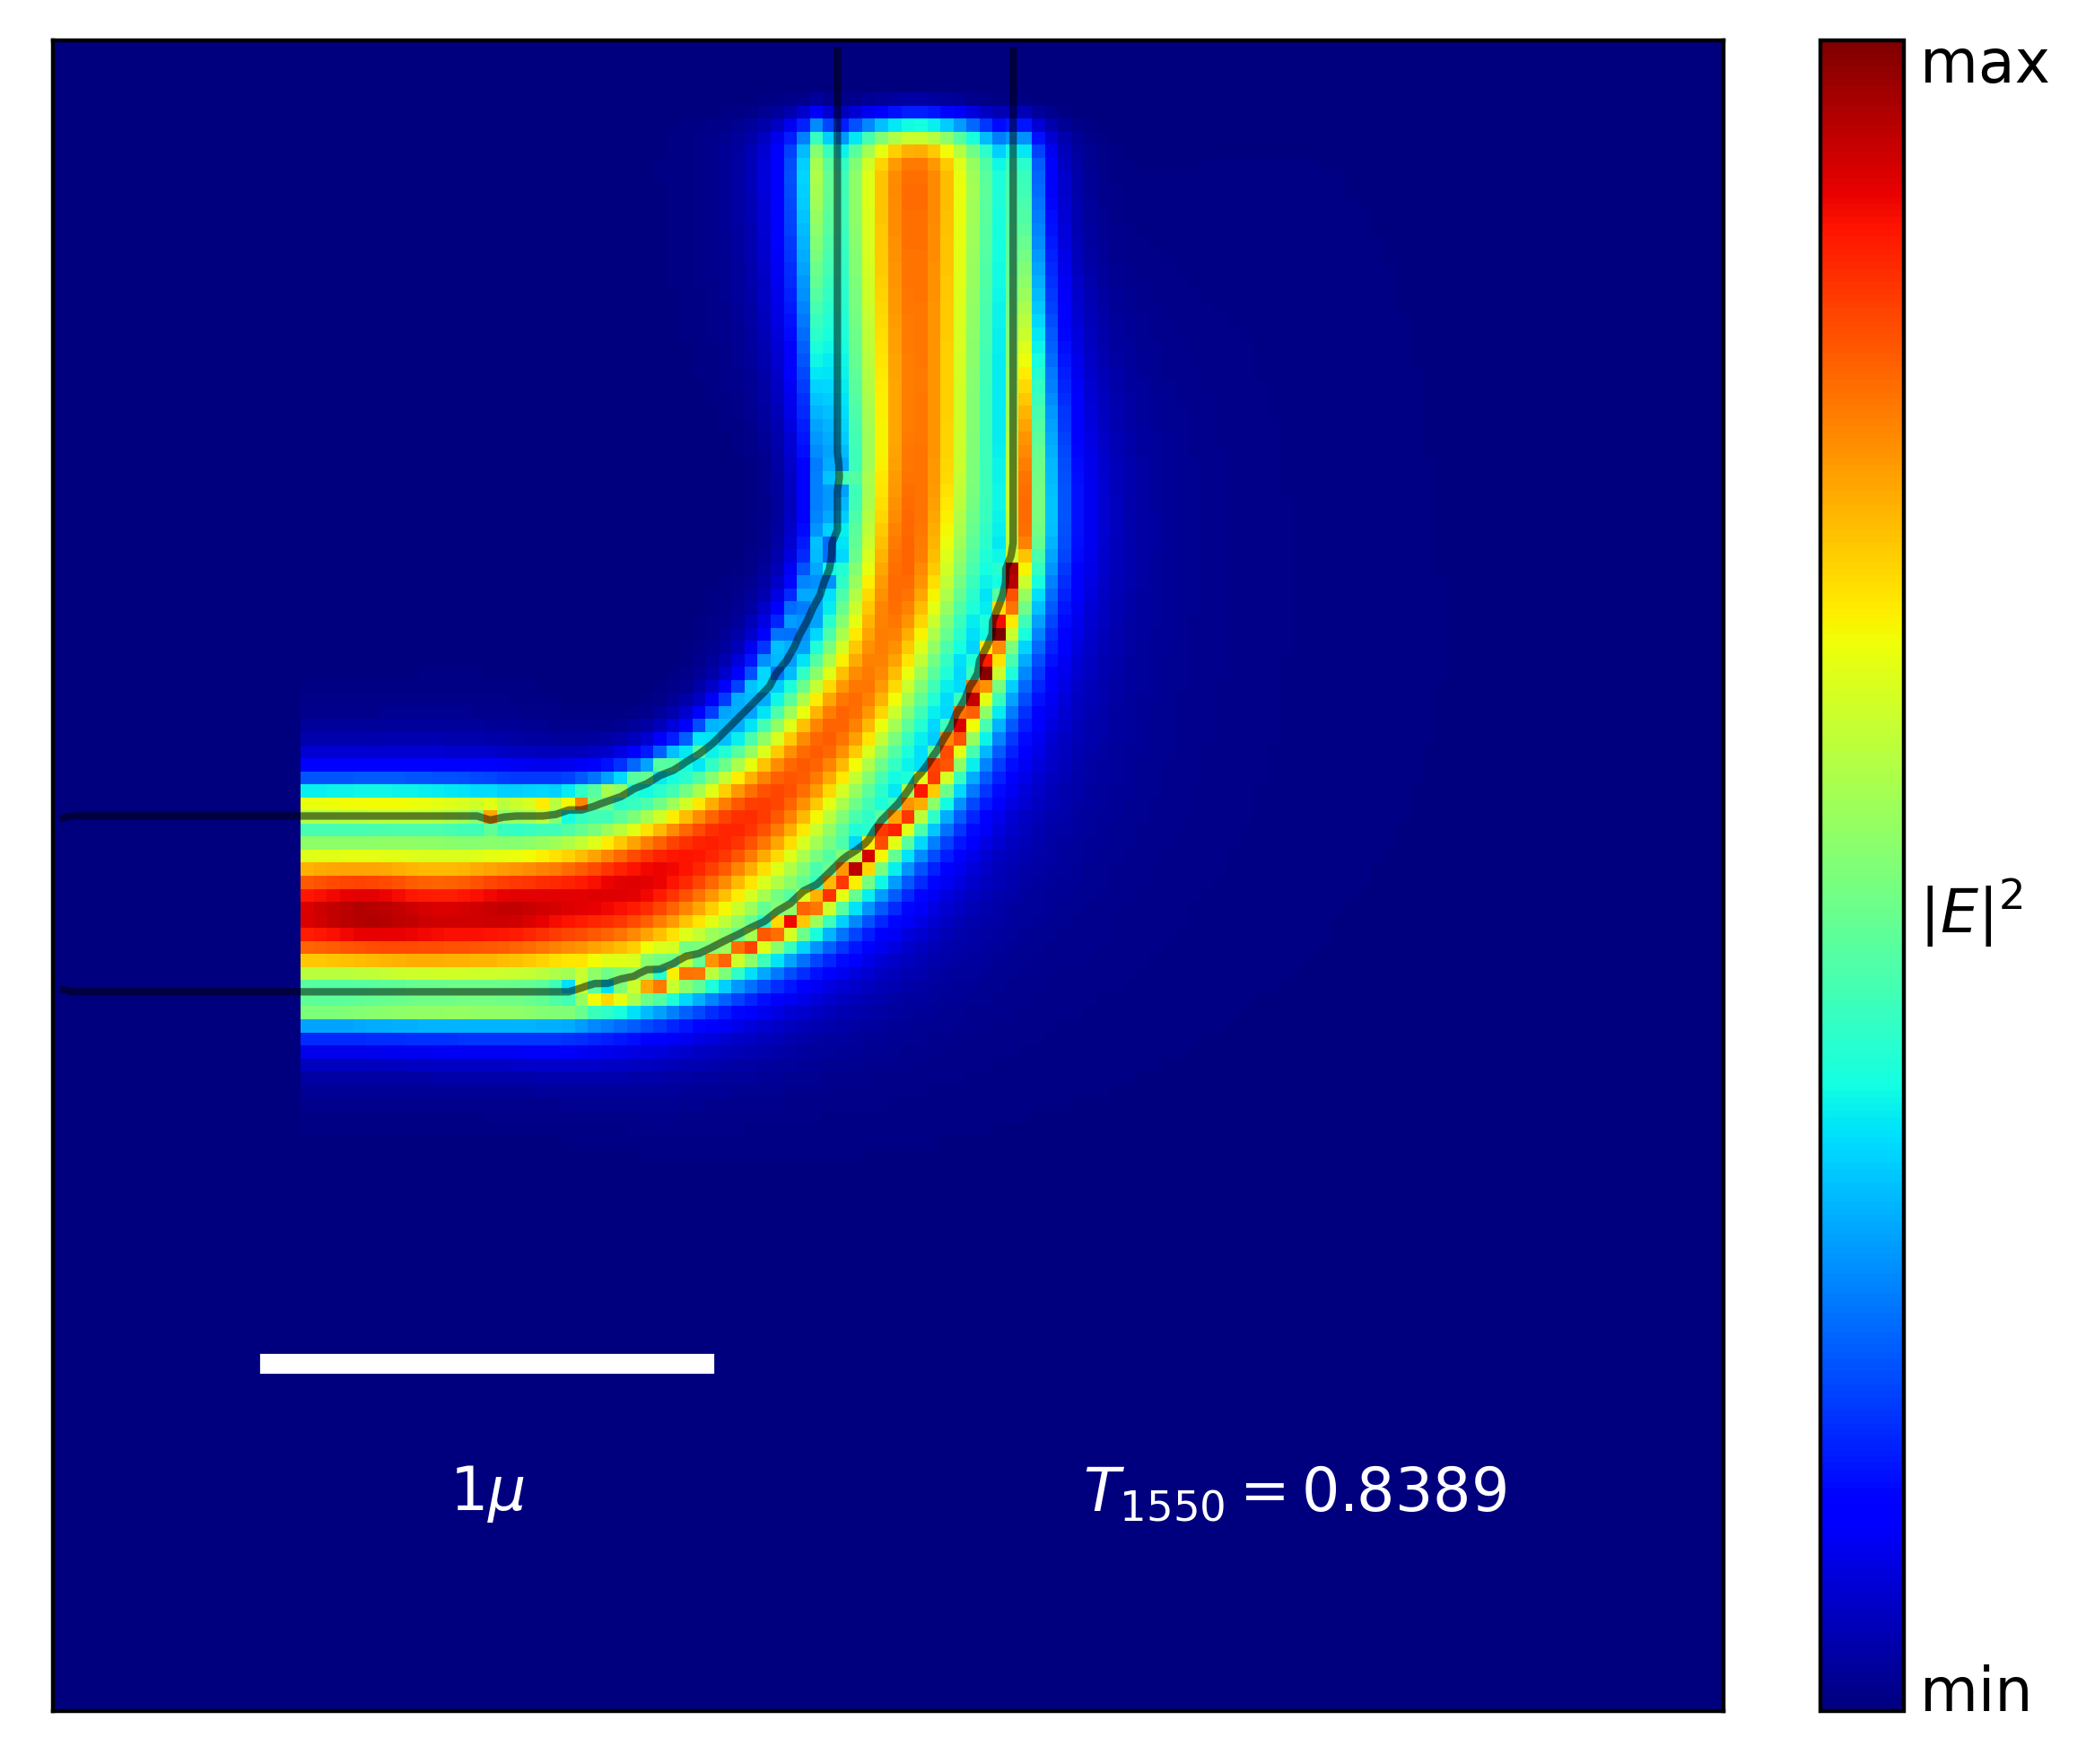
\includegraphics[scale=0.7]{image/theory/bend_field_dx30_px16_rint1000.png}
   \caption{Representación de $|\boldsymbol{E}|^2$ de un \emph{bend} de $1 \mu m$ de radio obtenido usando 3D FDFD bajo una resolución de $30 nm$.}
  \label{fig:efield}
\end{figure}


Tradicionalmente, un \emph{bend} consiste en una una guía de onda horizontal usada como entrada y
una guía de onda vertical usada como salida, estas son conectadas por una guía de onda con la forma de un
cuarto de circunferencia de radio $r$ y con el mismo grosor de las guías de onda de entrada y salida.
En la \autoref{fig:efield} se muestra un \emph{bend} tradicional de radio $r = 1 \mu m$.
Como se observa en la imagen, parte significativa de la energía se pierde en la región curva.
Esto se debe a que el radio de curvatura es muy pequeño, con un valor más grande (e.g. $r = 10 \mu m$) 
las pérdidas se vuelven casi nulas \citep{LukasChrostowski2010}.


Para evitar ambigüedades, dos puntos adicionales a remarcar son: 
(i) cuando nos referimos al radio estamos haciendo mención al radio medio de curvatura y 
(ii) todos los diseños mostrados en este trabajo tienen un profundidad de 220nm.

Observar en una gráfica el valor de $|\boldsymbol{E}|^2$ nos ayuda a entender el funcionamiento de un dispositivo.
Por otro lado, una manera de cuantificar que tan bien funciona un diseño es mediante el cálculo de la
transmitancia $(T)$.
Este valor se define como la relación entre la potencia del flujo que sale del dispositivo con la 
potencia del flujo que ingresa \citep{Christiansen2021}.

Seguidamente, sea $\lambda$ la longitud de onda de la entrada y $\boldsymbol{P}$ los parámetros que caracterizan al
diseño, denotaremos como $T_{\lambda}(\boldsymbol{P})$ a la transmitancia asociada al dispositivo obtenido con la
parametrización $\boldsymbol{P}$ en la longitud de onda $\lambda$. Luego, definimos la función objetivo 
($f_{obj}$) para un \emph{bend}, también conocido en el área como figura de mérito (FOM), 
mediante la siguiente ecuación \citep{Su2020}:

\begin{equation}
  f_{obj}(\boldsymbol{P}) = max \left \{ T_{1550} (\boldsymbol{P}) \right \}.
\label{eq:fom-bend}
\end{equation}

En síntesis, la idea detrás de estas definiciones es describir un \emph{bend} mediante una parametrización
$\boldsymbol{P}$
(\autoref{sec:parametrization}).
Luego, usando algoritmos de optimización, buscar entre las distintas combinaciones de los parámetros aquella configuración
que optimice la función $f_{obj}$ (\autoref{sec:alg-opt}).
De este modo, estaremos encontrando un diseño con una elevada transmitancia, es decir con un buen desempeño.

\subsection{\emph{Wavelength Demultiplexer} (WDM)}

Un WDM es un dispositivo fotónico que se encarga de guiar un haz de ondas de acuerdo a su longitud de onda.
Por ejemplo, estos pueden trabajar con dos longitudes de onda y guían las de una longitud por la guía de onda superior
y las de otra longitud por la guía de onda inferior.

Análogo al caso del \emph{bend}, utilizaremos la transmitancia para cuantificar el desempeño del dispositivo.
Pero, en el presente trabajo usaremos un WDM con dos guías de salida, por ello, utilizaremos como notación
$T_{\lambda}^{(1)}(\boldsymbol{P})$ para
representar la transmitancia en la guía de salida superior cuando se recibe un haz de longitud de onda
$\lambda$ en un diseño descrito por los parámetros $\boldsymbol{P}$ y $T_{\lambda}^{(2)}(\boldsymbol{P})$ para la guía de salida inferior.

\begin{figure}[ht]
  \centering
  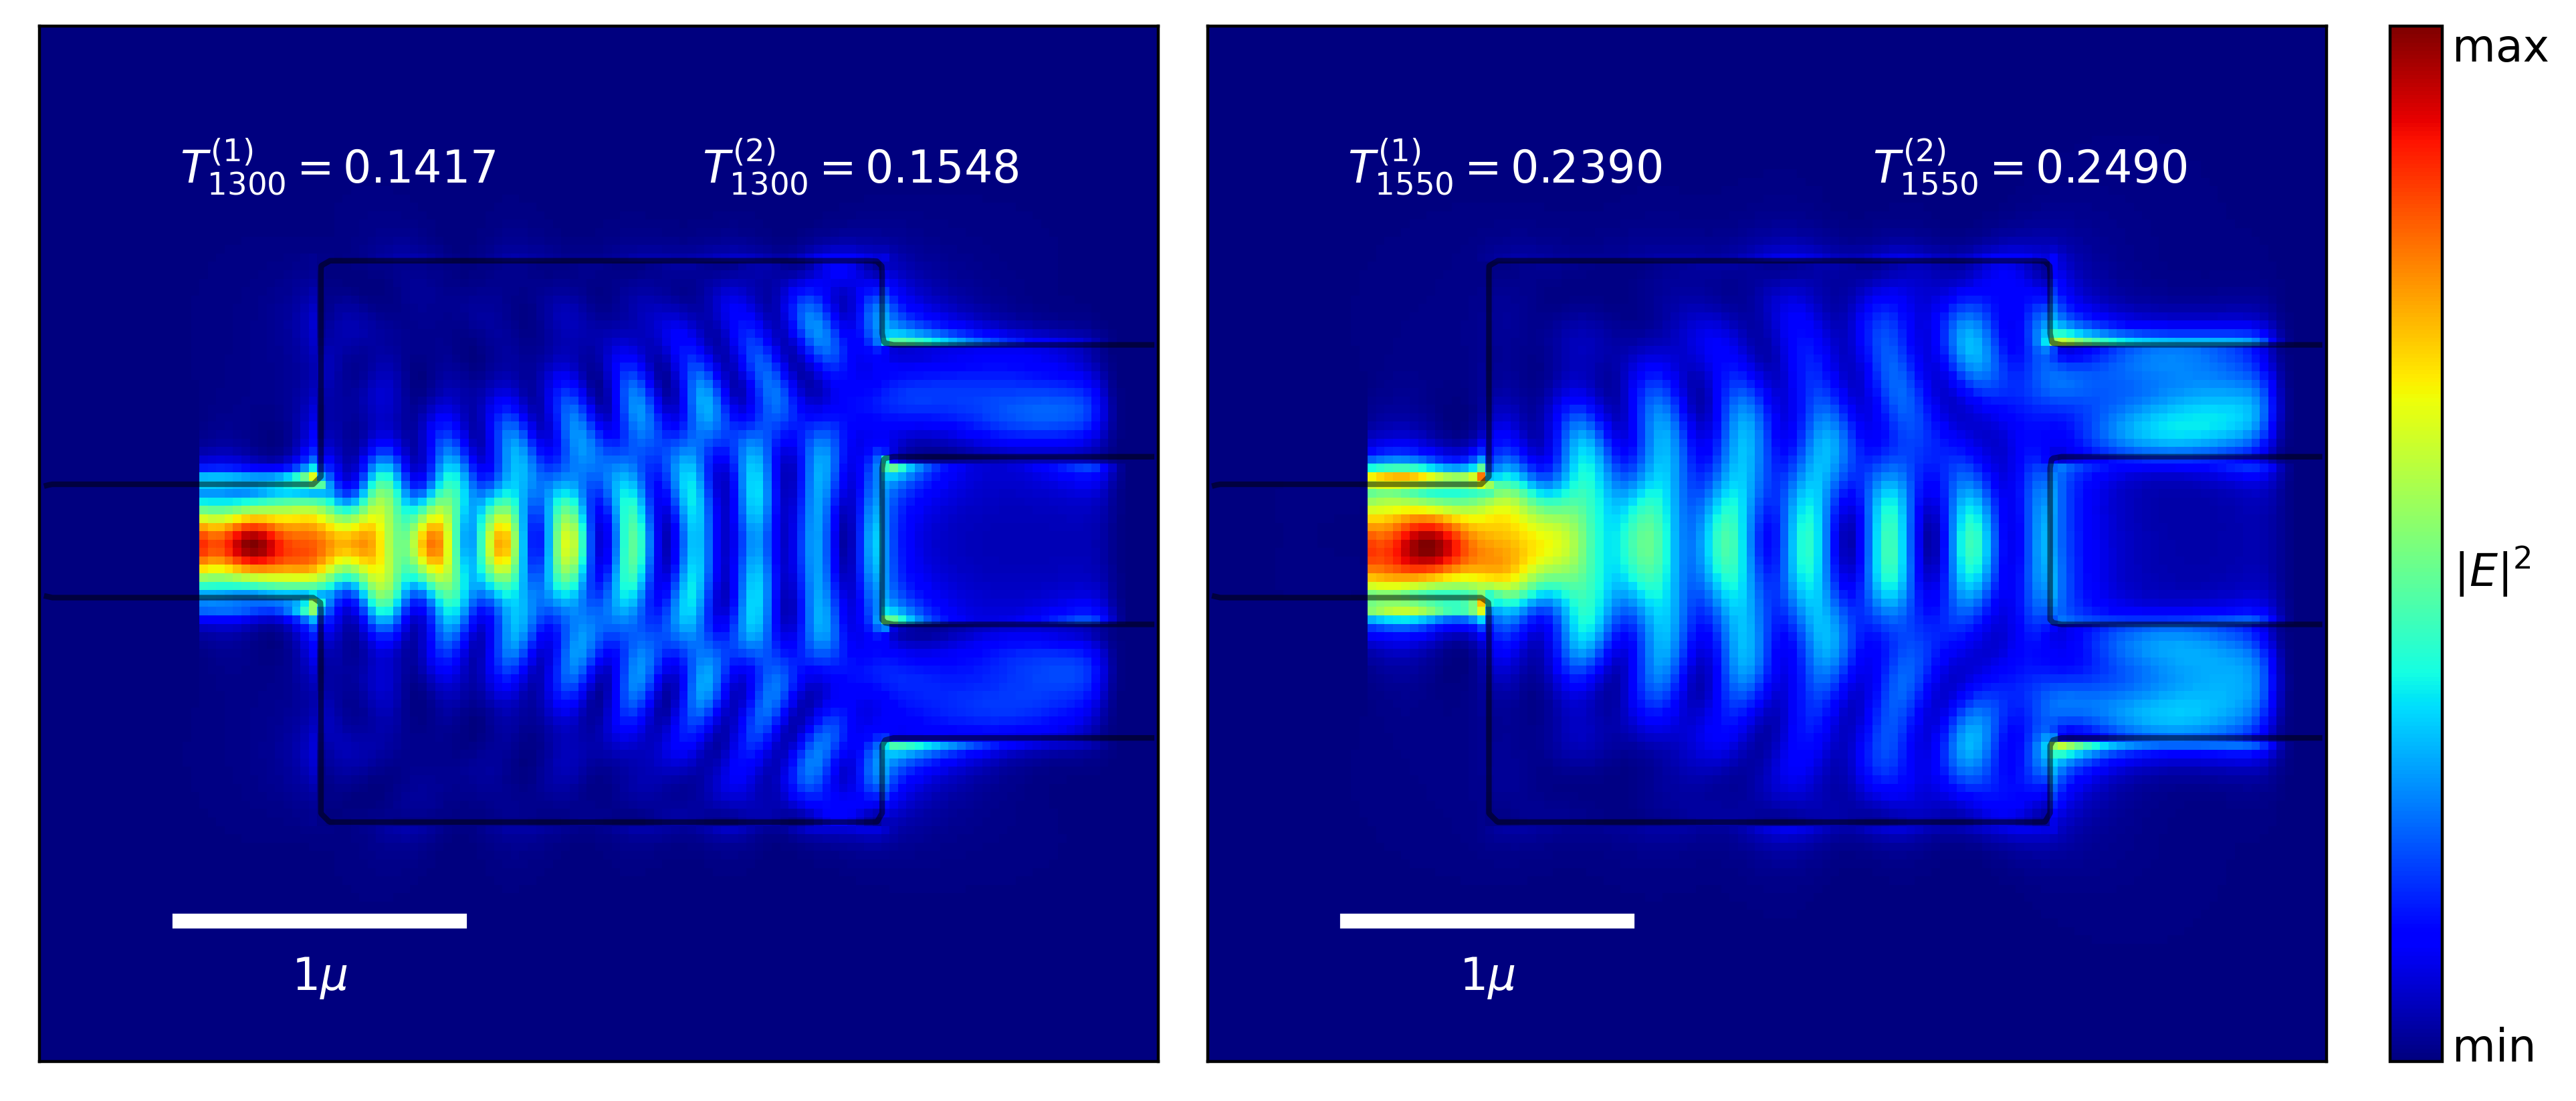
\includegraphics[scale=0.7]{image/theory/wdm_field_dx30_px16_px16.png}
  \caption{Representación de $|\boldsymbol{E}|^2$ de un WDM obtenido usando 3D FDFD bajo una resolución de $30 nm$.}
  \label{fig:efield-wdm}
\end{figure}

En la \autoref{fig:efield-wdm} se muestra un WDM donde las guías de onda son unidas por una región rectangular
de $2.0\mu m \times 2.0 \mu m$. En el lado izquierdo se muestra la representación de $|\boldsymbol{E}|^2$ cuando se usa 
como entrada un haz de ondas de $1300 nm$ de longitud, en el lado derecho la entrada es de $1550 nm$.
En ambos casos el diseño está funcionando más como un \emph{splitter} que como un WDM.
Un \emph{splitter} es un dispositivo fotónico que divide la potencia del flujo de la entrada por las guías
de salida en una determinada proporción. El diseño intuitivo para este dispositivo es el presentado en la imagen. Similar al caso del
\emph{bend}, con unas dimensiones un poco más grandes se puede conseguir pérdidas casi nulas de energía
\citep{LukasChrostowski2010}.
Sin embargo, como se observa en los valores de la transmitancia, este diseño intuitivo no es apropiado para un WDM.

Basándonos en \cite{Su2020}, definimos su FOM como

\begin{equation}
  f_{obj}(\boldsymbol{P}) = max \left \{ \frac{\left ( T_{1300}^{(1)}(\boldsymbol{P}) \right )^2  + 
                            \left ( 1 - T_{1300}^{(2)}(\boldsymbol{P}) \right )^2 +
                            \left ( 1 - T_{1550}^{(1)}(\boldsymbol{P}) \right )^2  + 
                            \left ( T_{1550}^{(2)}(\boldsymbol{P}) \right )^2 }{4}
                    \right \}.
\label{eq:fom-splitter}
\end{equation}

La \autoref{eq:fom-splitter} busca maximizar la transmitancia por la guía de onda superior y minimizarla para
la guía de onda inferior cuando se recibe una longitud de onda de $1300 nm$ y lo contrario para una longitud
de onda de $1550 nm$. Cabe destacar que la división por cuatro se realiza para asegurar que $f_{obj}$ solamente
tenga valores en el intervalo $[0, 1]$, al igual que sucede con la función objetivo del \emph{bend}.

La idea para optimizar un WDM es la misma descrita en la anterior sección. 
En el resto del capítulo se describe en más detalle los siguientes pasos necesarios para lograr esto.

\section{Parametrización}\label{sec:parametrization}

Tanto para el \emph{bend} como para el WDM se define una región de diseño
mediante una parametrización ($\boldsymbol{P}$) que pueda mapear un gran conjunto de dispositivos.
Una de la estrategias más populares para esta tarea es usar parametrización
basada en píxeles. Esta estrategia consiste en definir $\boldsymbol{P}$ como una matriz 
de $n$ filas y $m$ columnas con valores en el intervalo $[0, 1]$.
Al proceso de optimizar un dispositivo con esta parametrización se le conoce como optimización
topológica \citep{Molesky2018}.

\begin{figure}[h]
  \centering
  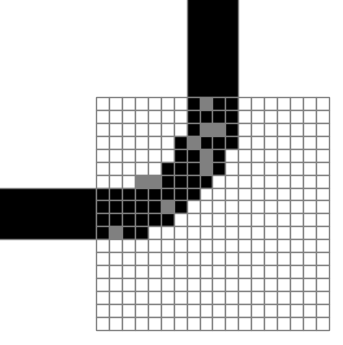
\includegraphics[scale=0.7]{image/theory/parametrization-pixeles.png}
  \caption{Parametrización basada en píxeles para un \emph{bend} definiendo $\boldsymbol{P}$ como una matriz de $18 \times 18$.}
  \label{fig:pixeles}
\end{figure}

A modo de ejemplo, en la \autoref{fig:pixeles} se ha definido la matriz $\boldsymbol{P}: [1, n] \times [1, m]
\to [0, 1]$ con $n = m = 18$ y se ha graficado sus valores
usando escala gris (0 corresponde al color blanco, 1 al negro y los demás valores a diferentes
intensidades del gris). De esta manera observamos como $\boldsymbol{P}$ logra definir la geometría de un
diseño.
Adicionalmente, conforme se incrementa el valor de $n$ y $m$ se logra definir detalles con mayor precisión.


Sin embargo, lo anterior solo nos permite describir la geometría de los diseños, no sus propiedades.
Además, no queda claro qué representan las regiones grises.
Por ello, para describir las propiedades del diseño es necesario asociar a $\boldsymbol{P}$ alguna propiedad física.
Esto lo realizamos calculando la permitividad ($\boldsymbol{\varepsilon}$) mediante la siguiente ecuación:

\begin{equation}
  \boldsymbol{\varepsilon}(x, y) = \varepsilon_{Si} + (1 - \boldsymbol{P}(x, y))
  \varepsilon_{SiO_2} \, \mid \, x \in [1, n] \land y \in [1, m],
\label{eq:permitivity}
\end{equation}

\noindent donde $\varepsilon_{Si} = 3.48^2$ es la permitividad del silicio ($Si$) y
$\varepsilon_{SiO_2} = 1.44^2$ es la permitividad del óxido de silicio ($SiO_2$).
De esta manera, la celda ubicada en la fila $x$, columna $y$ de la geometría descrita por 
$\boldsymbol{P}(x, y)$ tiene una permitividad de valor $\boldsymbol{\varepsilon}$(x, y).

Con la \autoref{eq:permitivity} estamos asociando a cada rectángulo de la geometría descrita por
$\boldsymbol{P}$ un valor de permitividad en el rango 
$[\varepsilon_{SiO2} = 1.44^2, 3.48^2 = \varepsilon_{Si}]$.
De esta manera, $\boldsymbol{P}(x, y) = 1$ describe que el rectángulo ubicado en la posición $(x, y)$ es de
$Si$,
un valor de $\boldsymbol{P}(x, y) = 0$ describe la presencia de $SiO_2$ y 
$0 < \boldsymbol{P}(x, y) < 1$ hace referencia
a algún material cuya permitividad es $\boldsymbol{\varepsilon}(x, y)$.

No obstante, un inconveniente de lo descrito es que $\boldsymbol{P}$ puede mapear a materiales inexistestes
(regiones grises),
mayor detalle de esta dificultad se estudia
en la \autoref{sec:transformations}.
Por otro lado, con la descripción de la permitividad ya podemos calcular los campos eléctricos con lo
cual se puede obtener el valor de $f_{obj}$ definido para el \emph{bend} y WDM.
Por esta razón se realizan simulaciones electromagnéticas y se resuelven las inversas de las 
ecuaciones de Maxwell, esto permite obtener los campos eléctricos \citep{Su2020}.
Afortunadamente, para este proceso se puede utilizar distintos programas que implementan diversos 
métodos numéricos para realizar los cálculos (\autoref{sec:simulation}).

\section{Simulación}\label{sec:simulation}

Una vez tenemos definido un dispositivo con regiones fijas (guías de onda) y una
región de diseño (descrita por la parametrización), es necesario incorporar
tres elementos adicionales \citep{Oskooi2010, Su2020}:

\begin{enumerate}

  \item \textbf{Fuente:} Suele representarse como un rectángulo en un plano perpendicular al flujo
    que pasa por el lugar donde este se ubica. Simula la emición de un haz de ondas por el diseño.

  \item \textbf{Monitores:} Suelen representarse como un rectángulo similar a la fuente.
    Capturan información en su ubicación (e.g. valores del campo eléctrico).

  \item \textbf{\emph{Perfectly Matched Layer} (PML):} Representan las condiciones de frontera en la simulación. 
    Se utilizan para limitar el espacio donde se deberá realizar las simulaciones computacionales.

\end{enumerate}

\begin{figure}[ht]
  \centering
  \subfigure[Vista frontal]
    {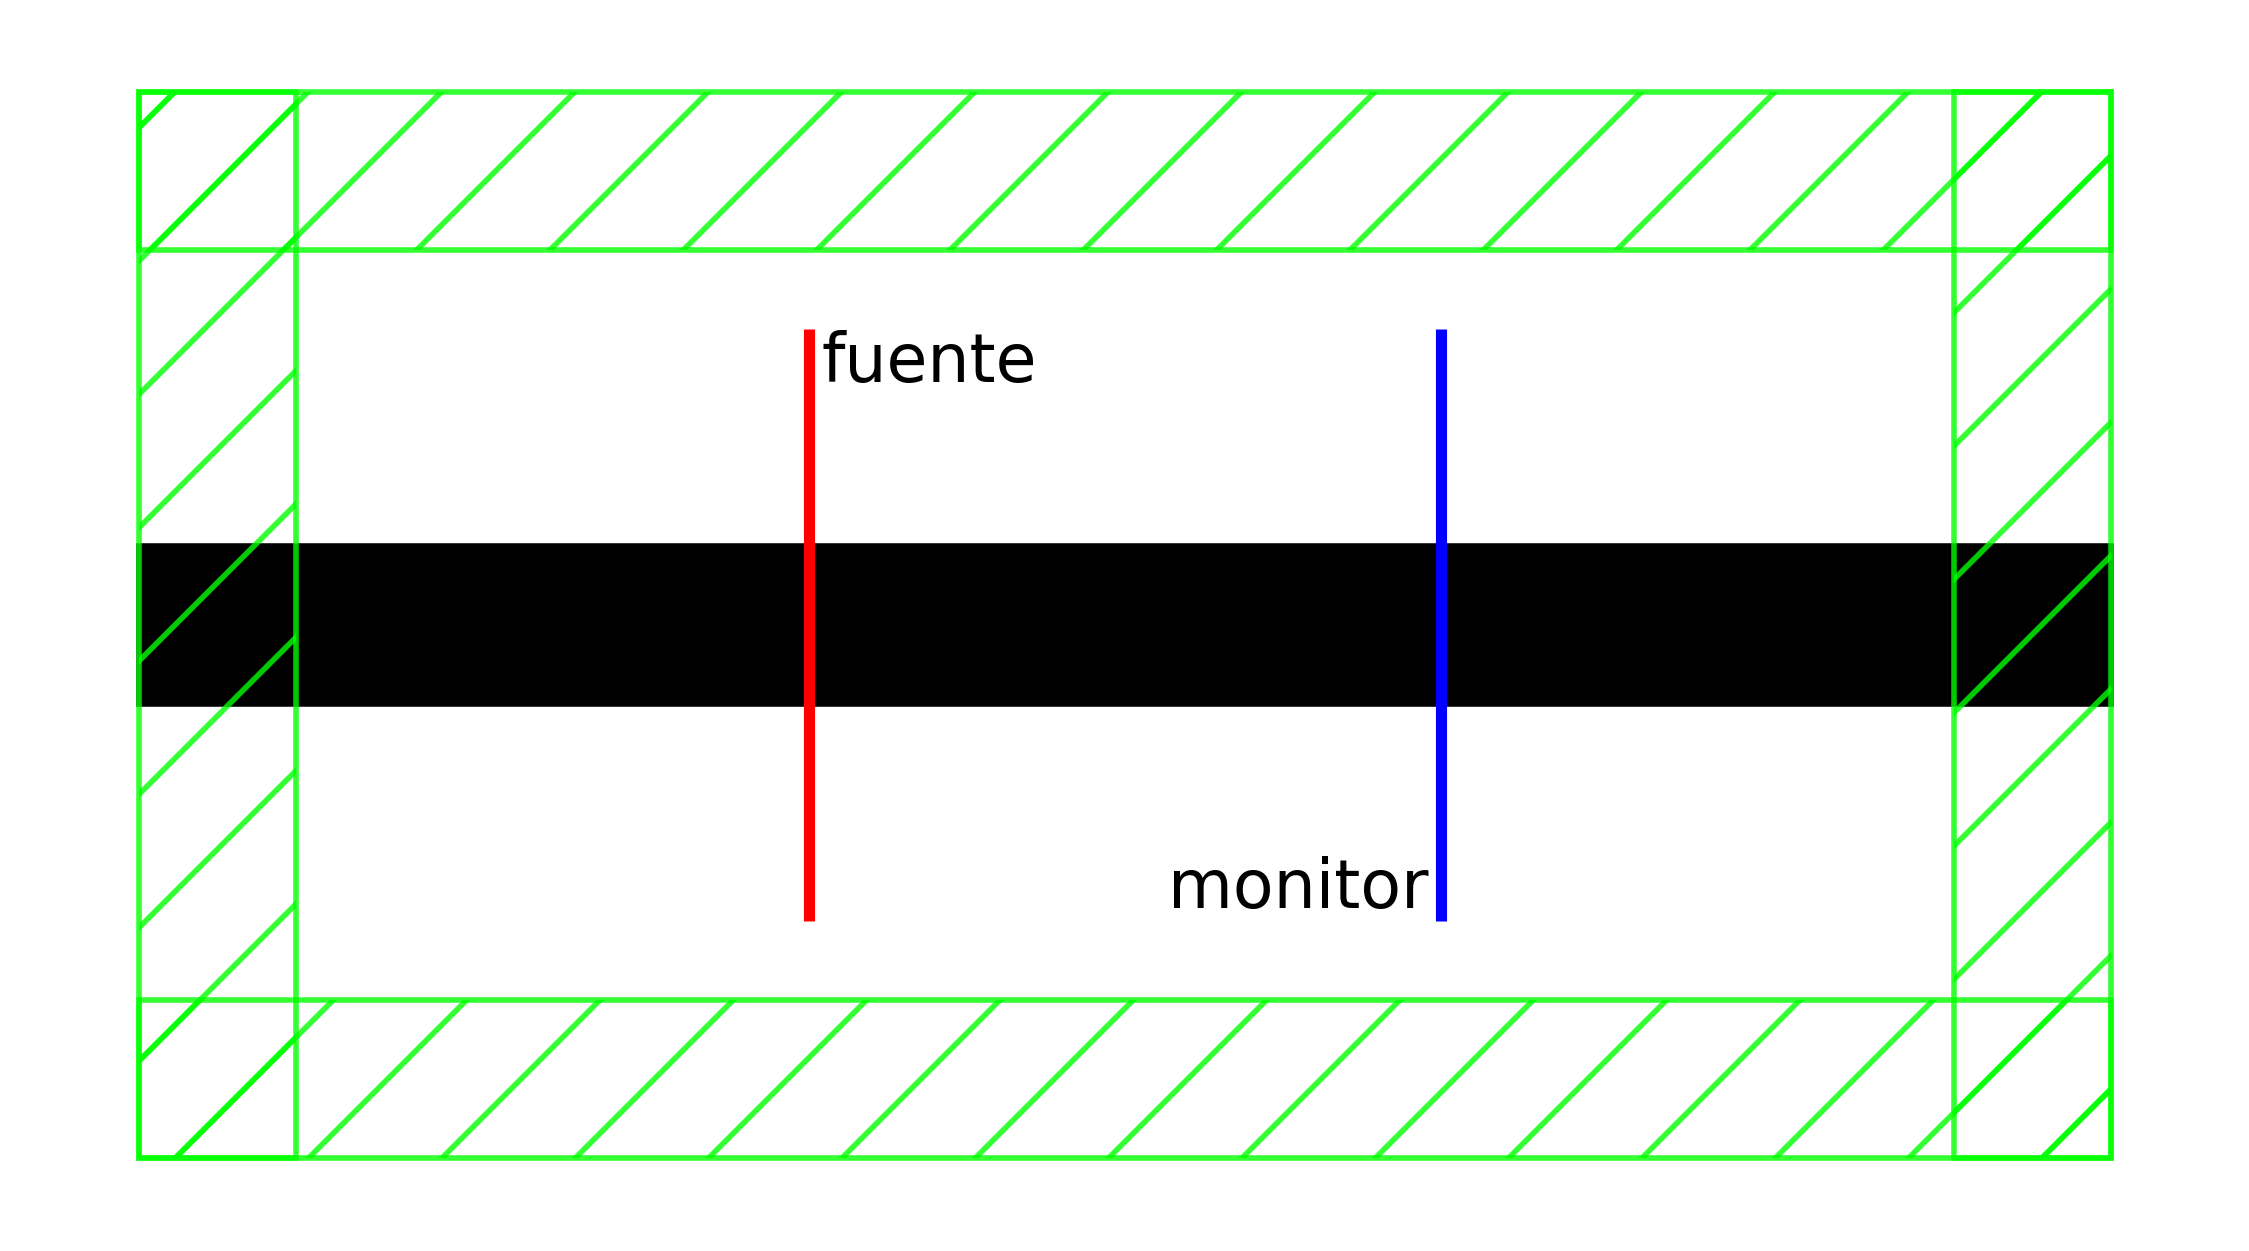
\includegraphics[width=0.45\textwidth]{image/theory/simulation.png}}
  \hfill
  \subfigure[Vista lateral]
    {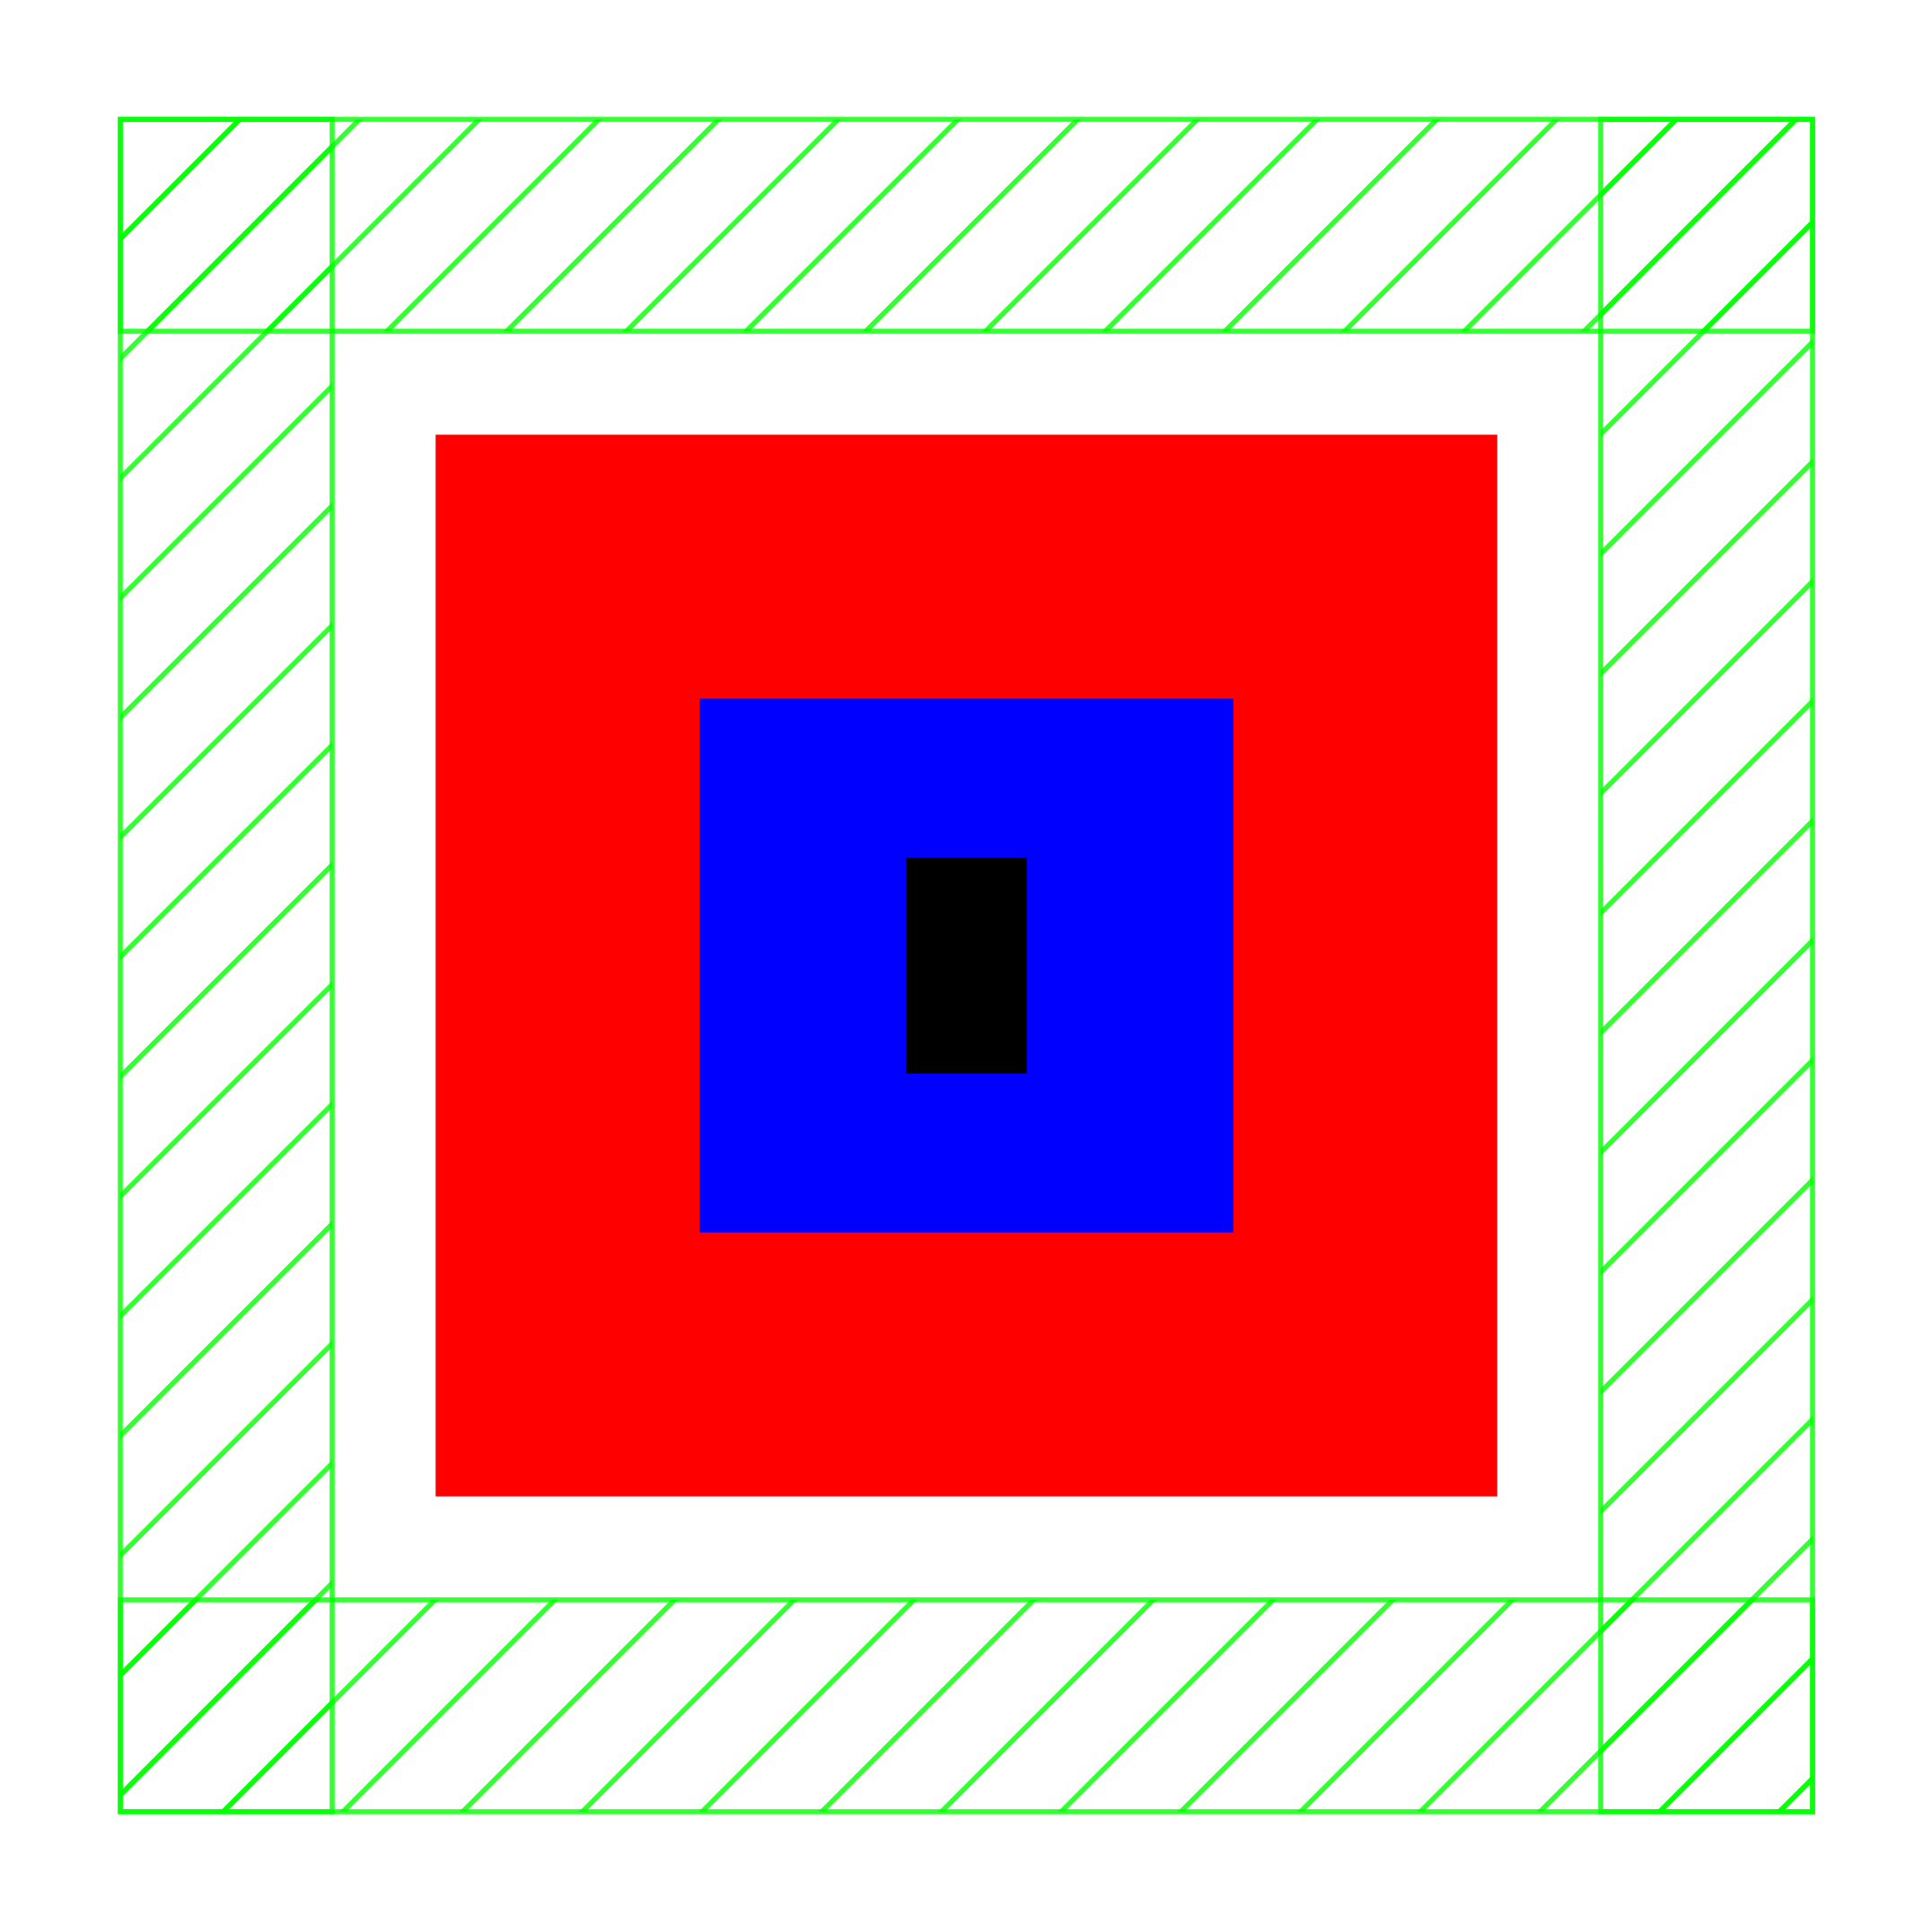
\includegraphics[width=0.45\textwidth]{image/theory/simulation-top.png}}

  \caption{Configuración de simulación para una guía de onda.}
  \label{fig:waveguide}
\end{figure}

En la \autoref{fig:waveguide} se ilustra una guía de onda con los elementos mencionados.
El rectángulo de color negro representa la guía de onda, la región roja la fuente, 
la región azul el monitor y lo verde el PML.
Guiándonos de la figura de la izquierda, al realizar una simulación con esta configuración 
el flujo iría de la región roja a la región azul.
Sin embargo, este seguiría expandiéndose por la guía de onda hasta llegar a la región verde (PML).
En palabras sencillas, podemos interpretar el PML como una caja que permite aislar nuestro sistema.
Por otro lado, la figura de la derecha representa el mismo diseño pero desde una vista lateral 
(recordemos que son diseños en 3D).
Aquí podemos evidenciar como la fuente y el monitor son representados por rectángulos, no por rectas.

Siguiendo lo descrito, podemos utilizar diversos programas para configurar y ejecutar 
simulaciones de un \emph{bend} y WDM.
Una alternativa es usar SPINS-B junto a Maxwell-B, paquetes de Python de código
abierto.
Estos paquetes funcionan bajo una arquitectura cliente-servidor donde SPINS-B es el cliente y Maxwell-B es el servidor.

Por un lado, SPINS-B permite configurar diseños (fuente, monitores, PML, parametrización, región de diseño, etc) y solicitar al servidor que obtenga sus propiedades.
Un aspecto interesante de este paquete es que trabaja con bloques llamados nodos.
Estos representan operaciones fundamentales como suma, resta, multiplicación, etc.
Luego, el programa guarda nuestra función objetivo ($f_{obj}$) usando un grafo que tiene estos nodos de vértices.
Así, SPINS-B permite calcular de forma eficiente
(usando un número de simulaciones independiente de las dimensiones de $\boldsymbol{P}$) 
el valor de $\nabla f_{obj}(\boldsymbol{P})$ mediante diferenciación automática \citep{Su2020, Mykel2019}.

Por otro lado, Maxwell-B implementa un método numérico conocido como \emph{finite-difference frequency domain}
(FDFD) para resolver numéricamente las ecuaciones de Maxwell y obtener así determinadas propiedades
de los diseños que recibe.
Es importante destacar que la implementación de esta librería es en GPUs de NVIDIA y permite
aprovechar múltiples GPUs a la vez.


Un último detalle a señalar es que para las simulaciones debemos definir su resolución,
esto lo representamos con el parámetro $dx$. 
Su valor se utiliza para discretizar nuestro espacio de
simulación en una malla de cubos de dimensiones $dx \times dx \times dx$.
En general, cuanto más pequeño es este valor
los resultados son más precisos, pero la cantidad de memoria y el tiempo de
simulación se incrementan considerablemente.

\section{Transformaciones}\label{sec:transformations}

En esta sección se discute dos transformaciones populares en optimización topológica
para imponer restricciones de fabricación en nuestreos diseños: (i) filtro por densidad y
(ii) proyección.

\subsection{Filtro por Densidad}

Antes de definir el filtro por densidad, necesitamos definir el concepto de bola cerrada.
Para ello, tenemos que definir el concepto de función distancia en nuestra matriz
de parametrización. Así, sea $x, x' \in [1, n] \land y, y' \in [1, m]$, definimos 
la distancia entre las posiciones $(x, y)$ y $(x', y')$ de la matriz $\boldsymbol{P}$ como:

\begin{equation}
  dis(x, y, x', y') = |x-x'|*psize_y+|y-y'|*psize_x,
  \label{eq:distance}
\end{equation}

\noindent donde $psize_x$ es el valor de la longitud horizontal que representa cada celda de $\boldsymbol{P}$
y $psize_y$ es el recíproco para la longitud vertical.

De esta manera, definimos la bola cerrada ($\overline{B}_{r}(x, y)$)  de centro $(x, y)$ y 
radio $0 < r$ mediante el siguiente conjunto:

\begin{equation}
  \overline{B}_{r}(x, y) = \{(x', y') | 1 \leq x' \leq n \land 1 \leq m \leq m \land 
  dis(x, y, x', y') \leq r\}.
  \label{eq:bola}
\end{equation}

Seguidamente, usando estos conceptos en la matriz $\boldsymbol{P}$
se define el filtro por densidad ($\widetilde{\boldsymbol{P}}$) mediante la ecuación:

\begin{equation}
  \widetilde{\boldsymbol{P}}(x, y) = \frac{\displaystyle\sum_{(x', y') \in \overline{B}_{r_f}(x, y)} w_{x, y}(x', y')
  A(x', y')\boldsymbol{P}(x', y')}
  {\displaystyle\sum_{(x', y') \in \overline{B}_{r_f}(x, y)} w_{x, y}(x', y') A(x', y')},
  \label{eq:densityfilter}
\end{equation}

\begin{equation}
  w_{x, y}(x', y') = max(0, r_f - dis(x, y, x', y')),
  \label{eq:hatbased}
\end{equation}

\noindent donde $A(x, y)$ es el área de la celda representada por $\boldsymbol{P}(x, y)$. 
Por otro lado, el concepto de mínimo radio de curvatura ($r_f$) hace referencia a que un diseño
se puede dibujar con una circunferencia de radio $r_f$.
El objetivo de la \autoref{eq:hatbased} es tratar de imponer este concepto al diseño.

Finalmente, de la \autoref{eq:densityfilter} podemos obtener el valor de su derivada parcial respecto al diseño
original calculando lo siguiente:

\begin{equation}
  \frac{\partial\widetilde{\boldsymbol{P}}(x, y)}{\partial \boldsymbol{P}(x^{*}, y^{*})} = \frac{w_{x, y}(x^{*},
  y^{*})A(x^{*}, y^{*})}
  {\displaystyle\sum_{(x', y') \in \overline{B}_{r_f}(x, y)} w_{x, y}(x', y') A(x', y')}.
  \label{eq:densityfiltergrad}
\end{equation}

\subsection{Proyección}

La proyección descrita en la sección anterior ayuda a obtener diseños que eviten regiones punteagudas;
sin embargo, esta transformación suele generar regiones grises.
Por este motivo, es común acompañar el filtro por densidad con una proyección 
($\widetilde{\widetilde{\boldsymbol{P}}}$) descrita como:

\begin{equation}
  \widetilde{\widetilde{\boldsymbol{P}}}(x, y) = \frac{\tanh (\beta \times \eta) + \tanh (\beta \times
  (\widetilde{\boldsymbol{P}}(x, y)
  - \eta))}{\tanh (\beta \times \eta) + \tanh (\beta \times (1 - \eta))},
  \label{eq:projection}
\end{equation}

\noindent donde $\eta$ y $\beta$ son números escalares. Para entender el impacto de estos parámetros
en la \autoref{eq:projection}, veamos la \autoref{fig:discretization}.
En la figura se está graficando esta ecuación con un valor fijo de $\eta = 0.5$ y distintos valores de
$\beta$.
Como podemos observar, con $\beta = 1$ tenemos prácticamente la función identidad y conforme aumenta
el valor de $\beta$ la función se aproxima más a una función escalonada con quiebre en $0.5$. 
En realidad, en general el quiebre se realiza en el valor que se le de a $\eta$.

    \begin{figure}[ht]
      \centering
      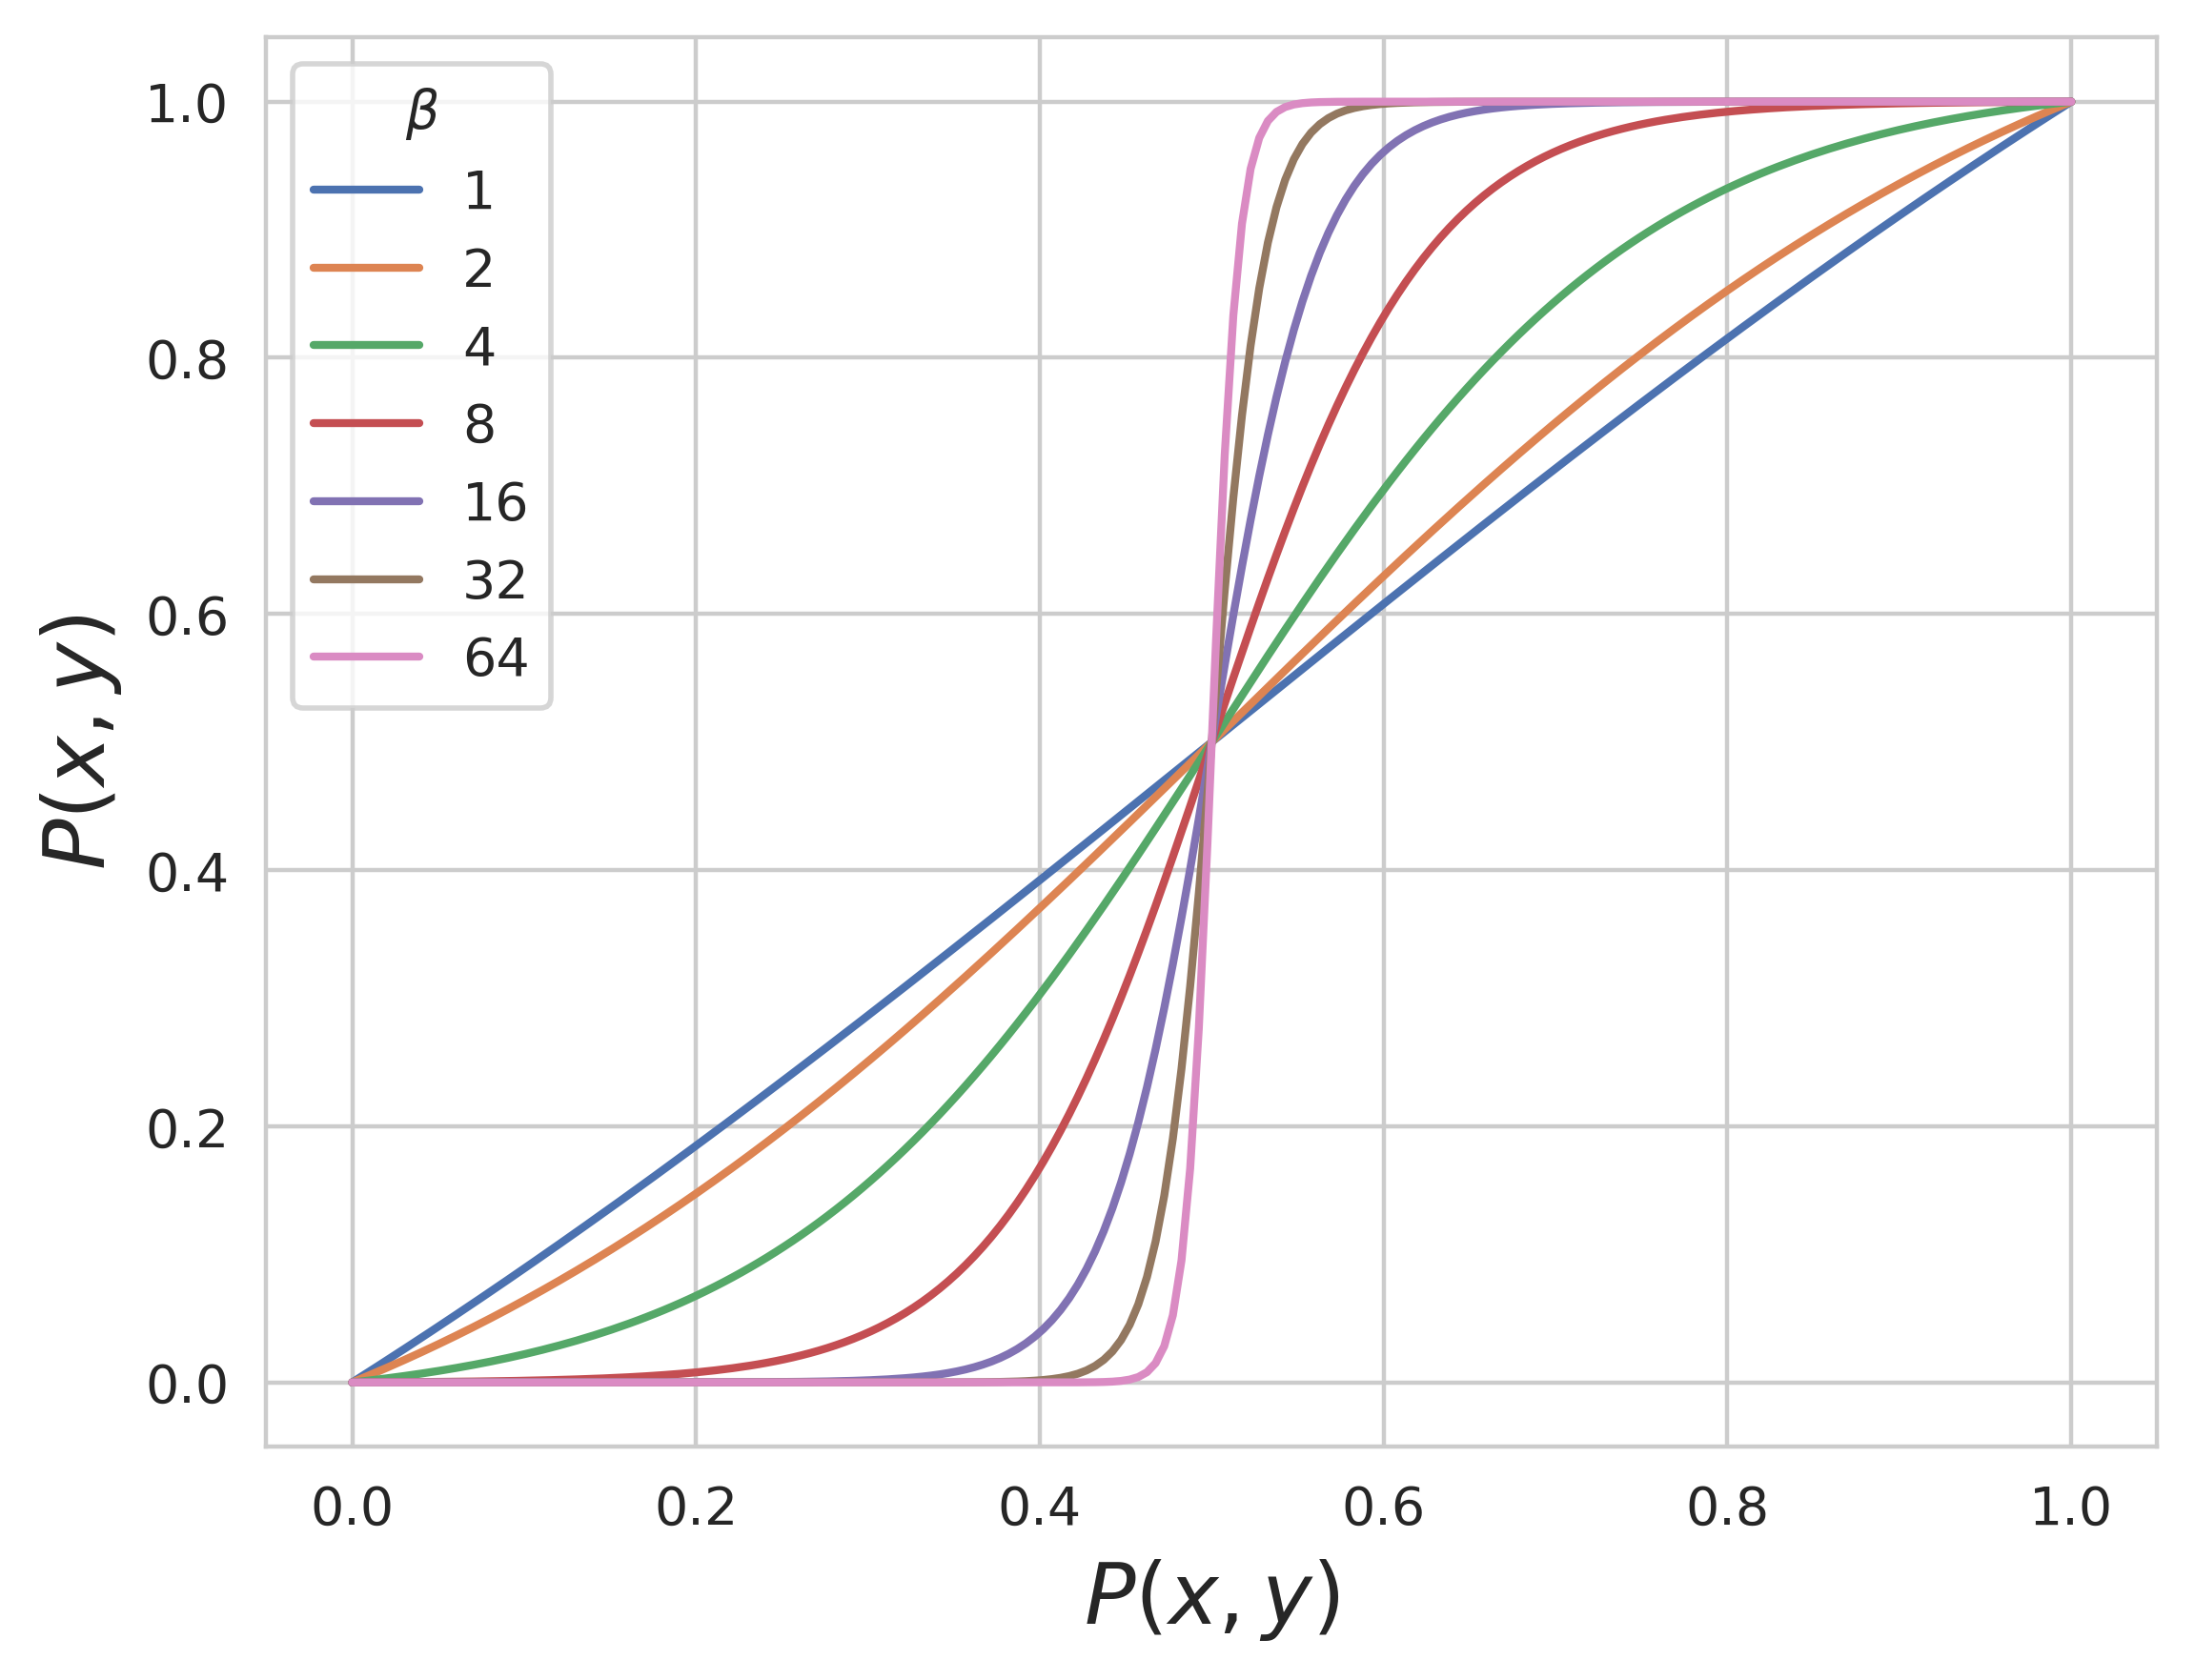
\includegraphics[scale=0.75]{image/theory/discretization.png}
      \caption{Transformación de proyección con $\eta = 0.5$ y distintos valores
      de $\beta$.}
      \label{fig:discretization}
    \end{figure}

Además, de la \autoref{eq:projection} podemos obtener el valor de su derivada parcial 
respecto al diseño $\widetilde{\boldsymbol{P}}$ mediante la siguiente ecuación:

\begin{equation}
  \frac{\partial\widetilde{\widetilde{\boldsymbol{P}}}(x, y)}{\partial \widetilde{\boldsymbol{P}}(x, y)} =
  \frac{(1 - \tanh^2 (\beta \times (\widetilde{\boldsymbol{P}}(x, y) - \eta))) \beta}
       {\tanh (\beta \times \eta) + \tanh (\beta \times (1 - \eta))}.
  \label{eq:projection-grad}
\end{equation}

\subsection{Aplicación de las Transformaciones}

\begin{figure}[ht]
  \centering
  % 1° row
  % P
  \subfigure[$\boldsymbol{P}$.]
  {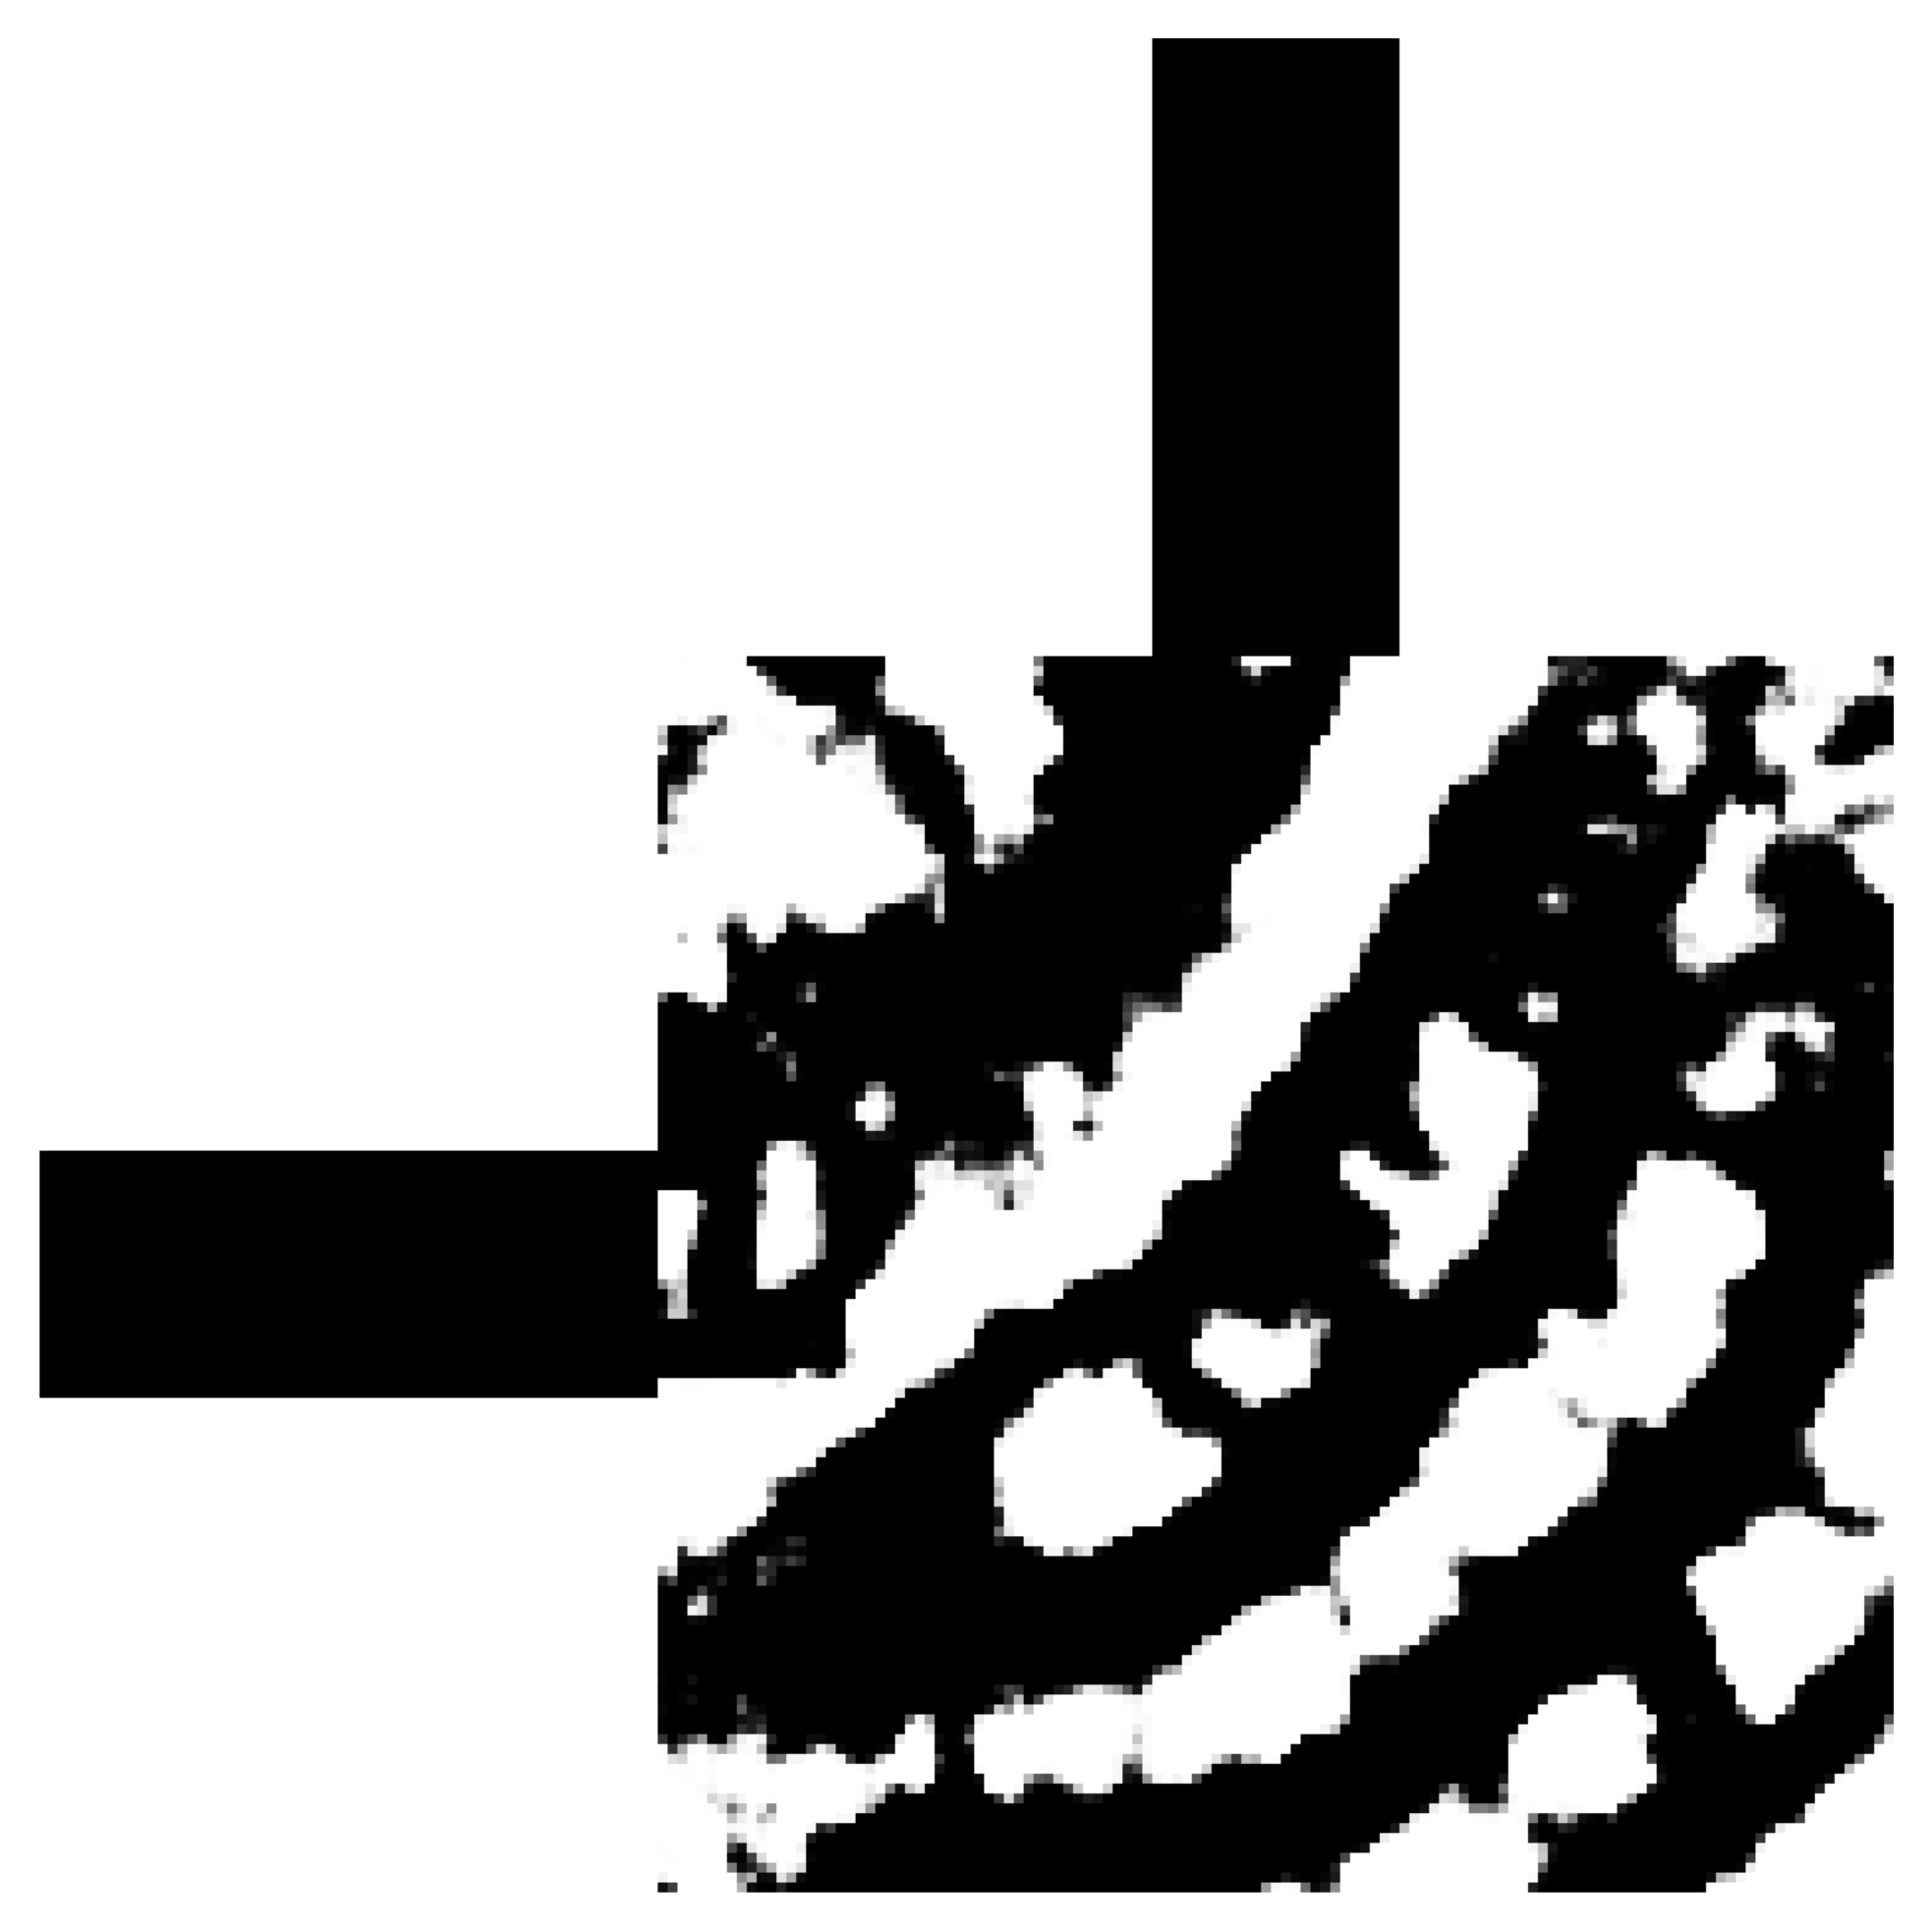
\includegraphics[width=0.4\textwidth]{image/theory/P.png}\label{subfig:P}}
  \hfill
  % filter P
  \subfigure[$\widetilde{\boldsymbol{P}}$ con $r_f = 80 nm$.]
  {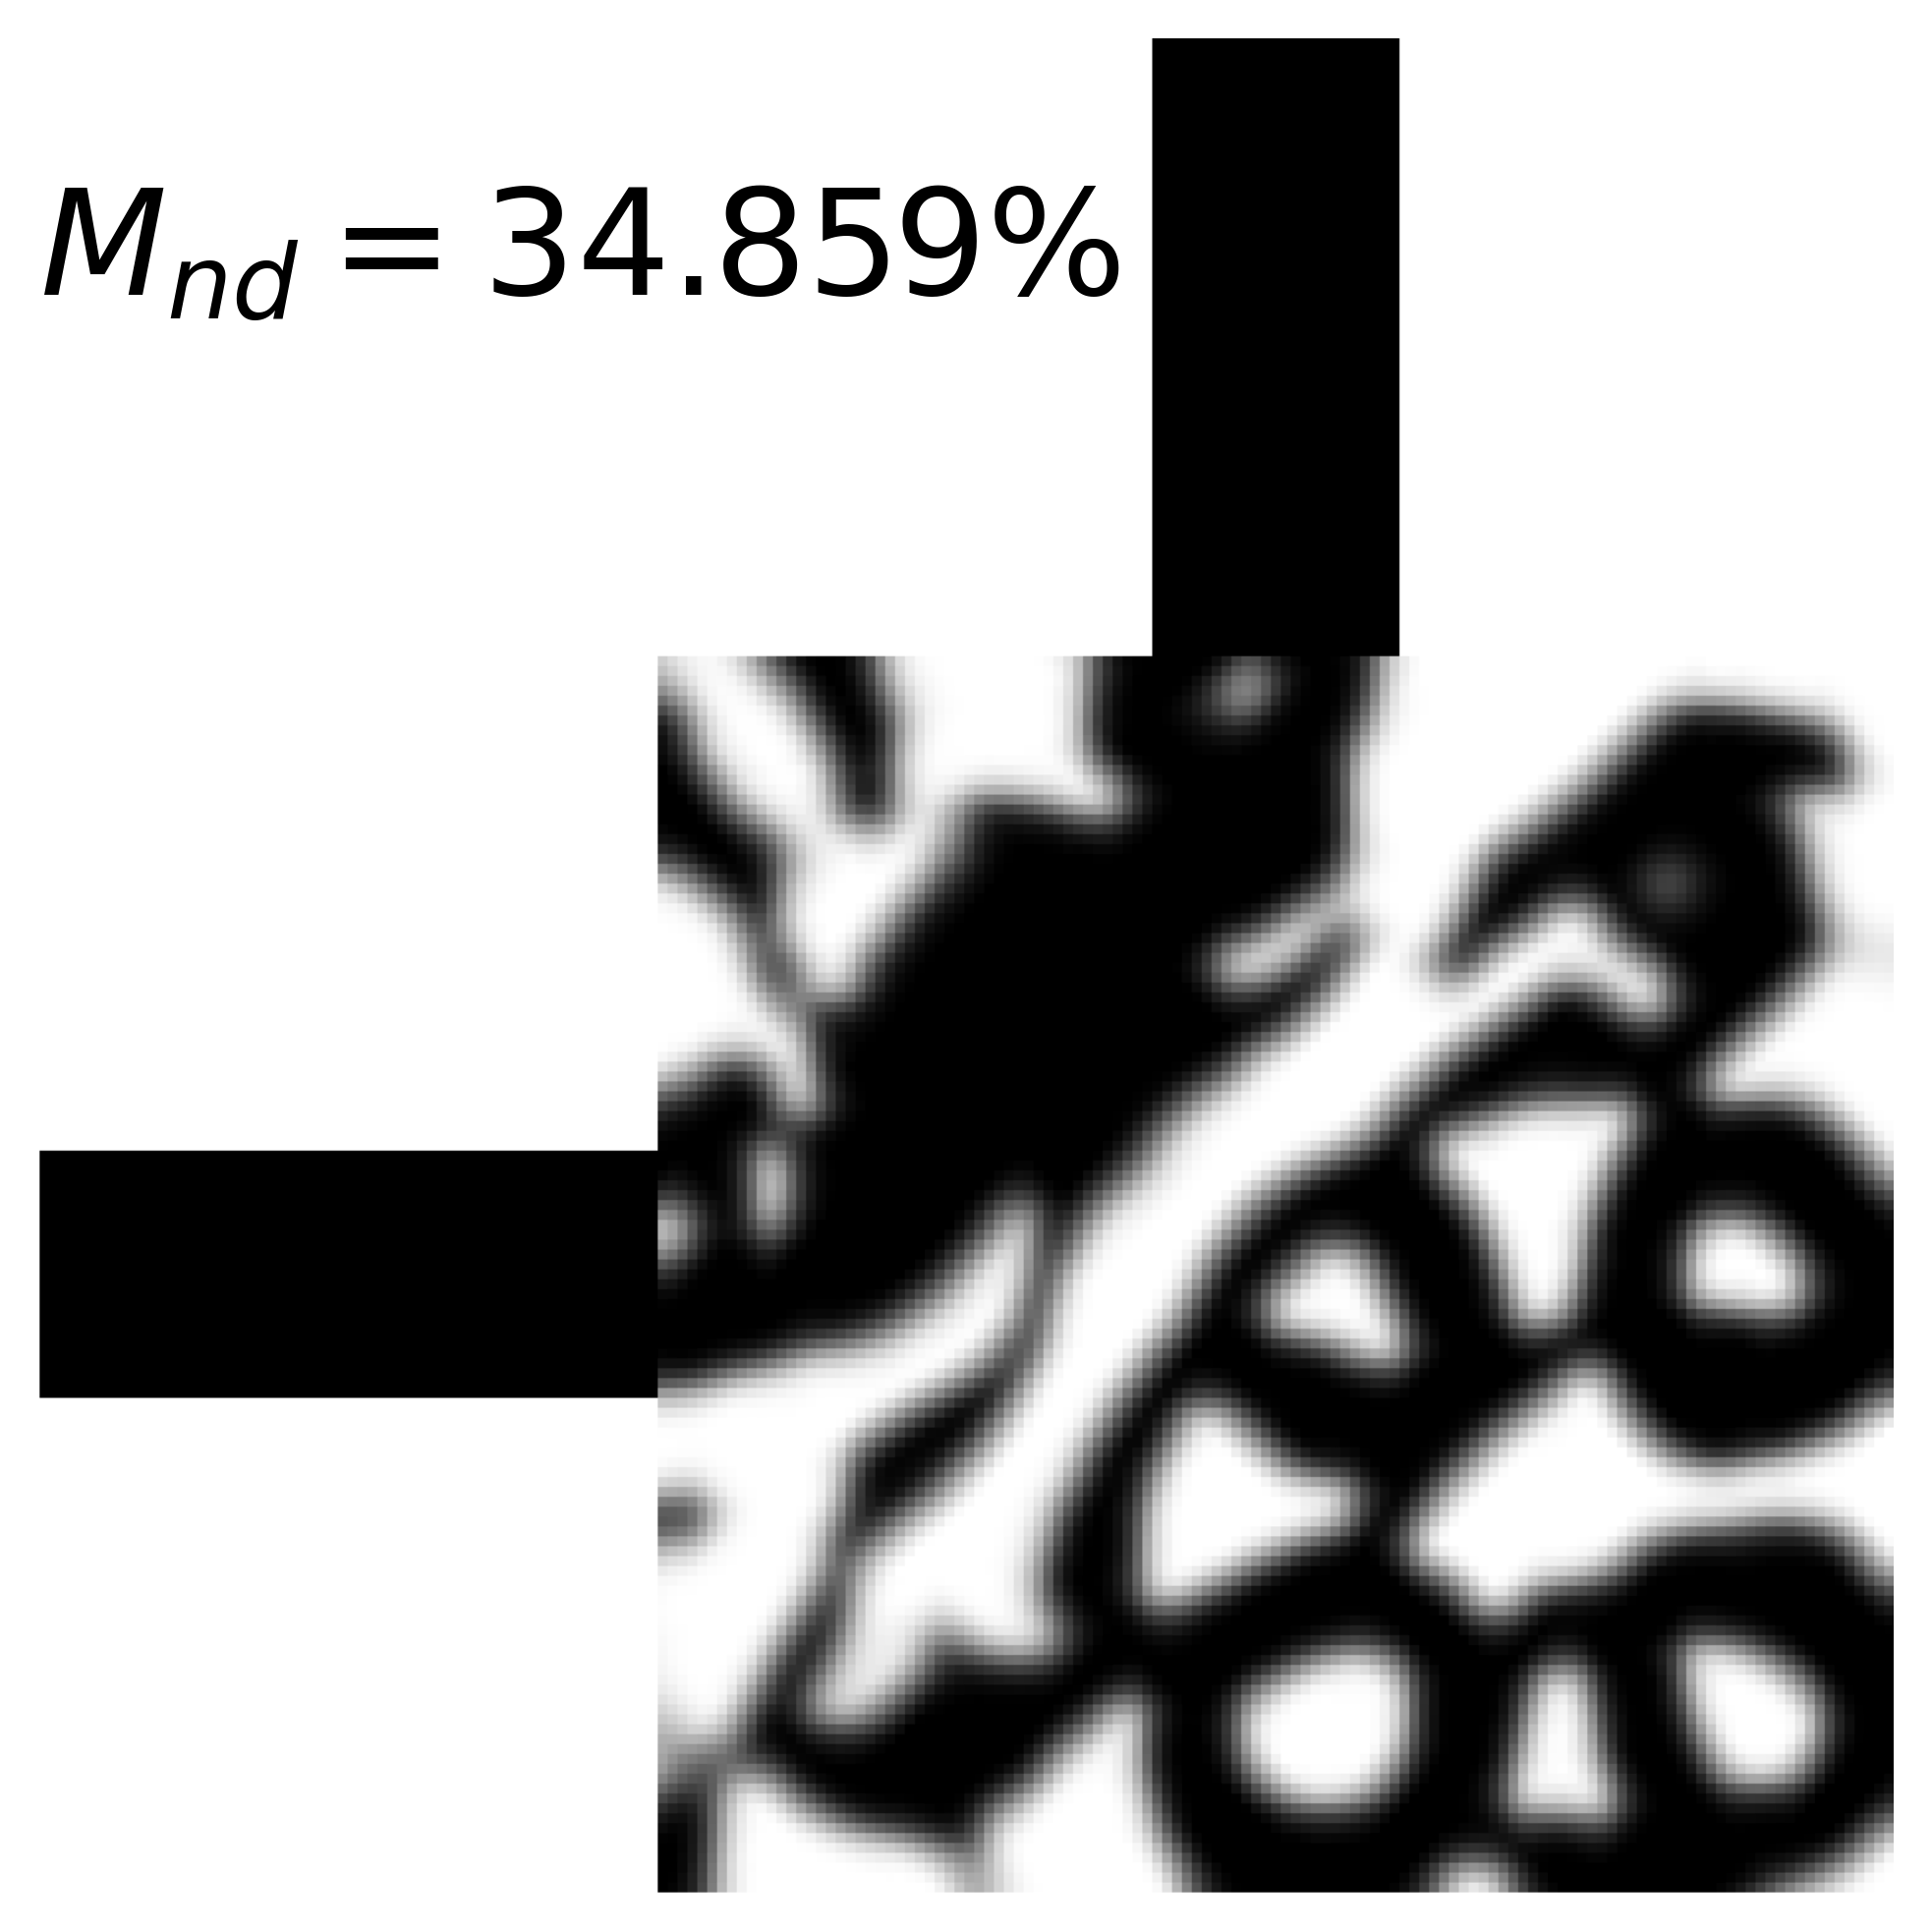
\includegraphics[width=0.4\textwidth]{image/theory/P_filter.png}\label{subfig:P_filter}}

  % 2° row
  \subfigure[$\widetilde{\widetilde{\boldsymbol{P}}}$ con $\eta_d = 0.3$ y $\beta = 2^6$.]
  {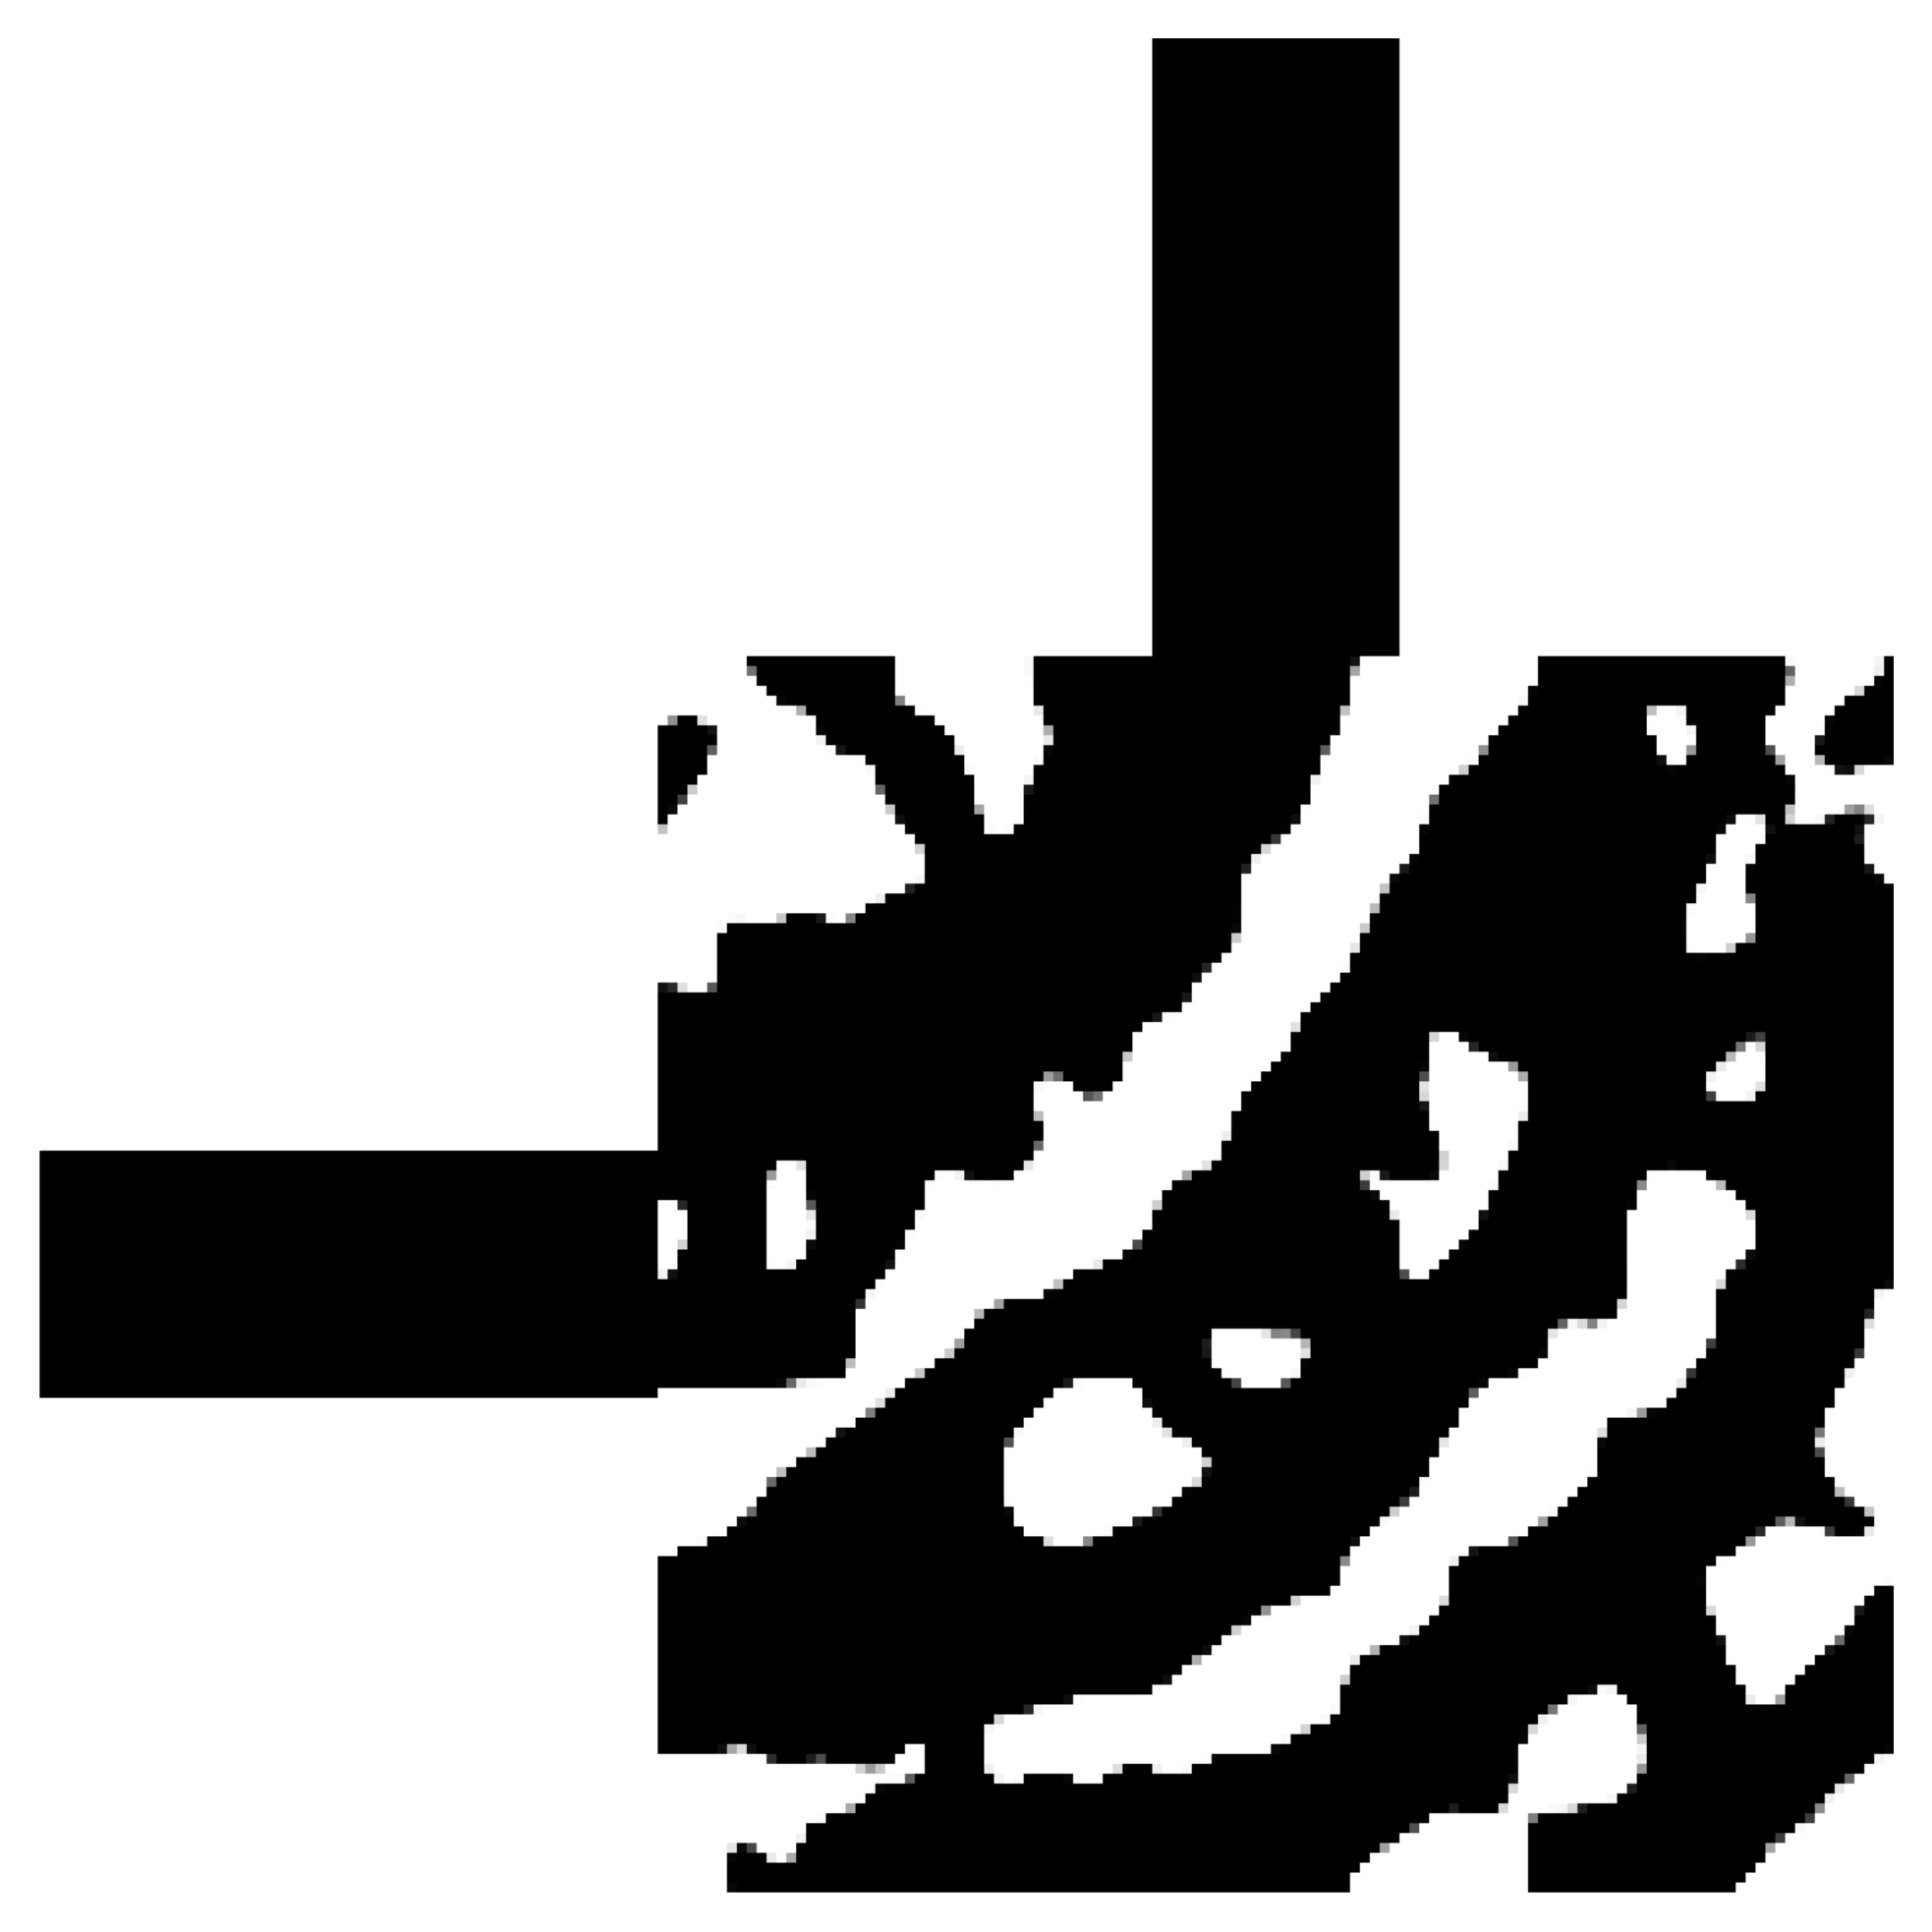
\includegraphics[width=0.3\textwidth]{image/theory/P_E_D.png}\label{subfig:P_E_D}}
  \hfill
  \subfigure[$\widetilde{\widetilde{\boldsymbol{P}}}$ con $\eta_i = 0.5$ y $\beta = 2^6$.]
  {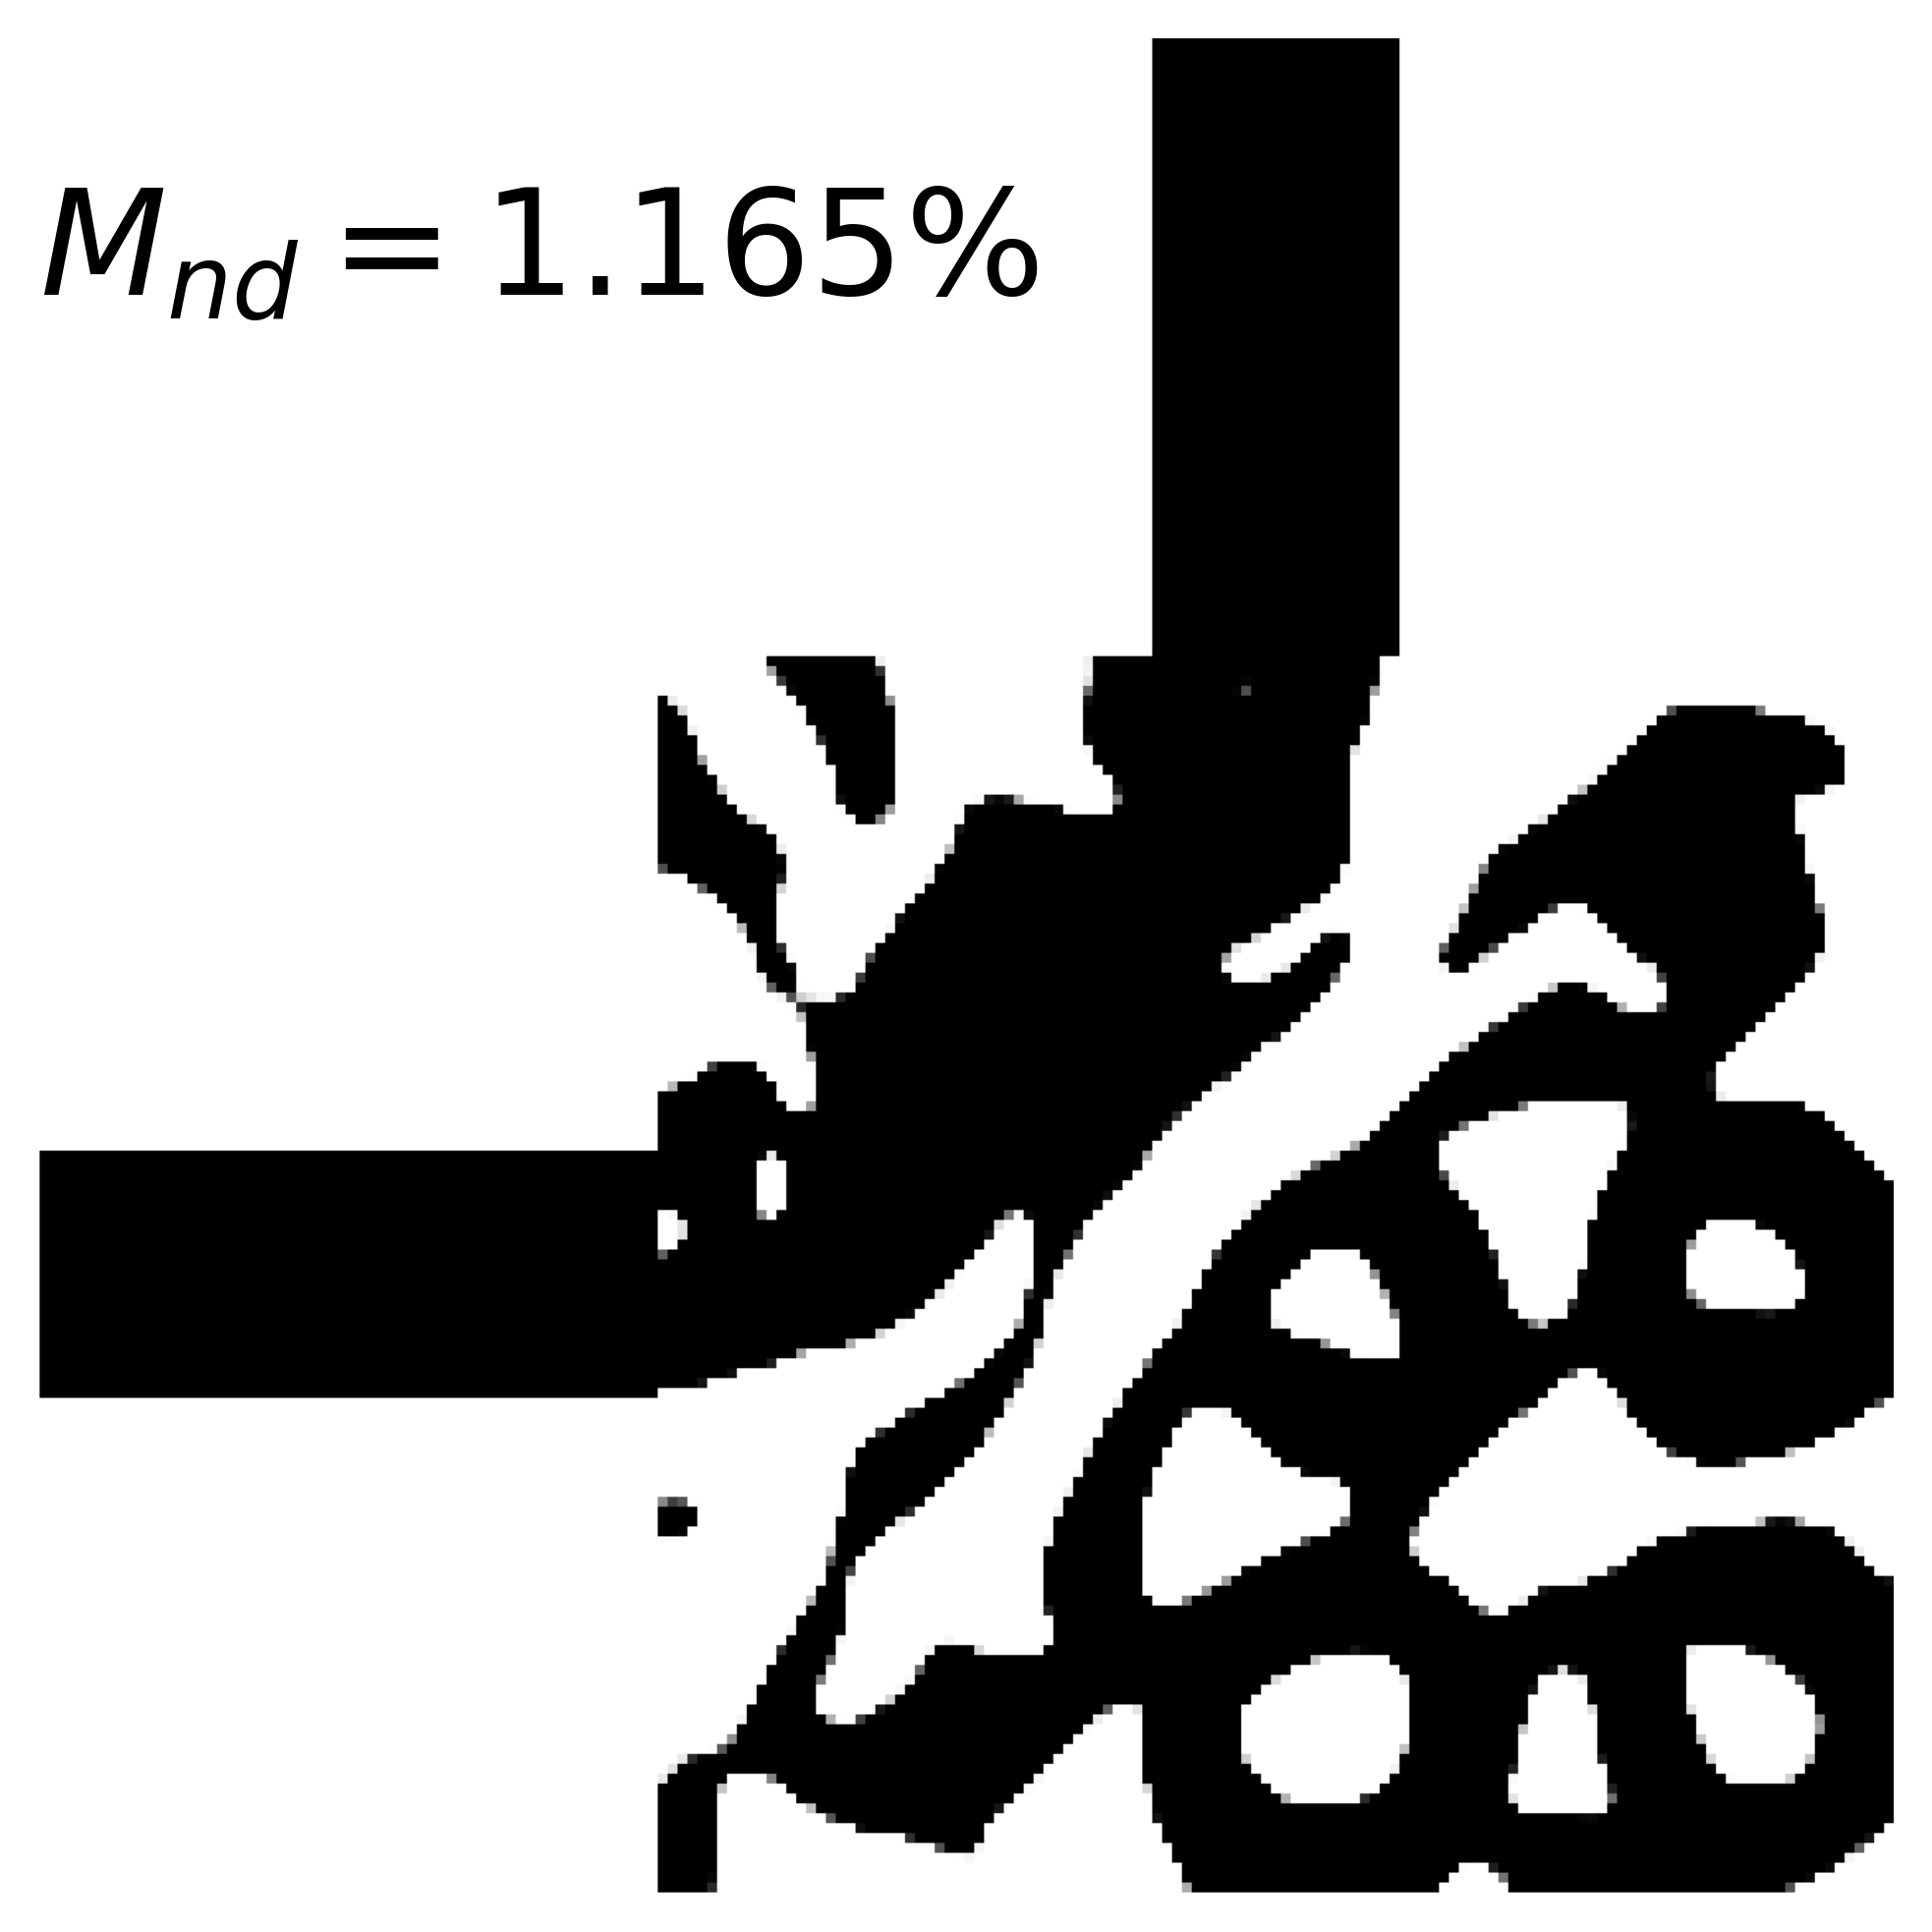
\includegraphics[width=0.3\textwidth]{image/theory/P_E_I.png}\label{subfig:P_E_I}}
  \hfill
  \subfigure[$\widetilde{\widetilde{\boldsymbol{P}}}$ con $\eta_e = 0.7$ y $\beta = 2^6$.]
  {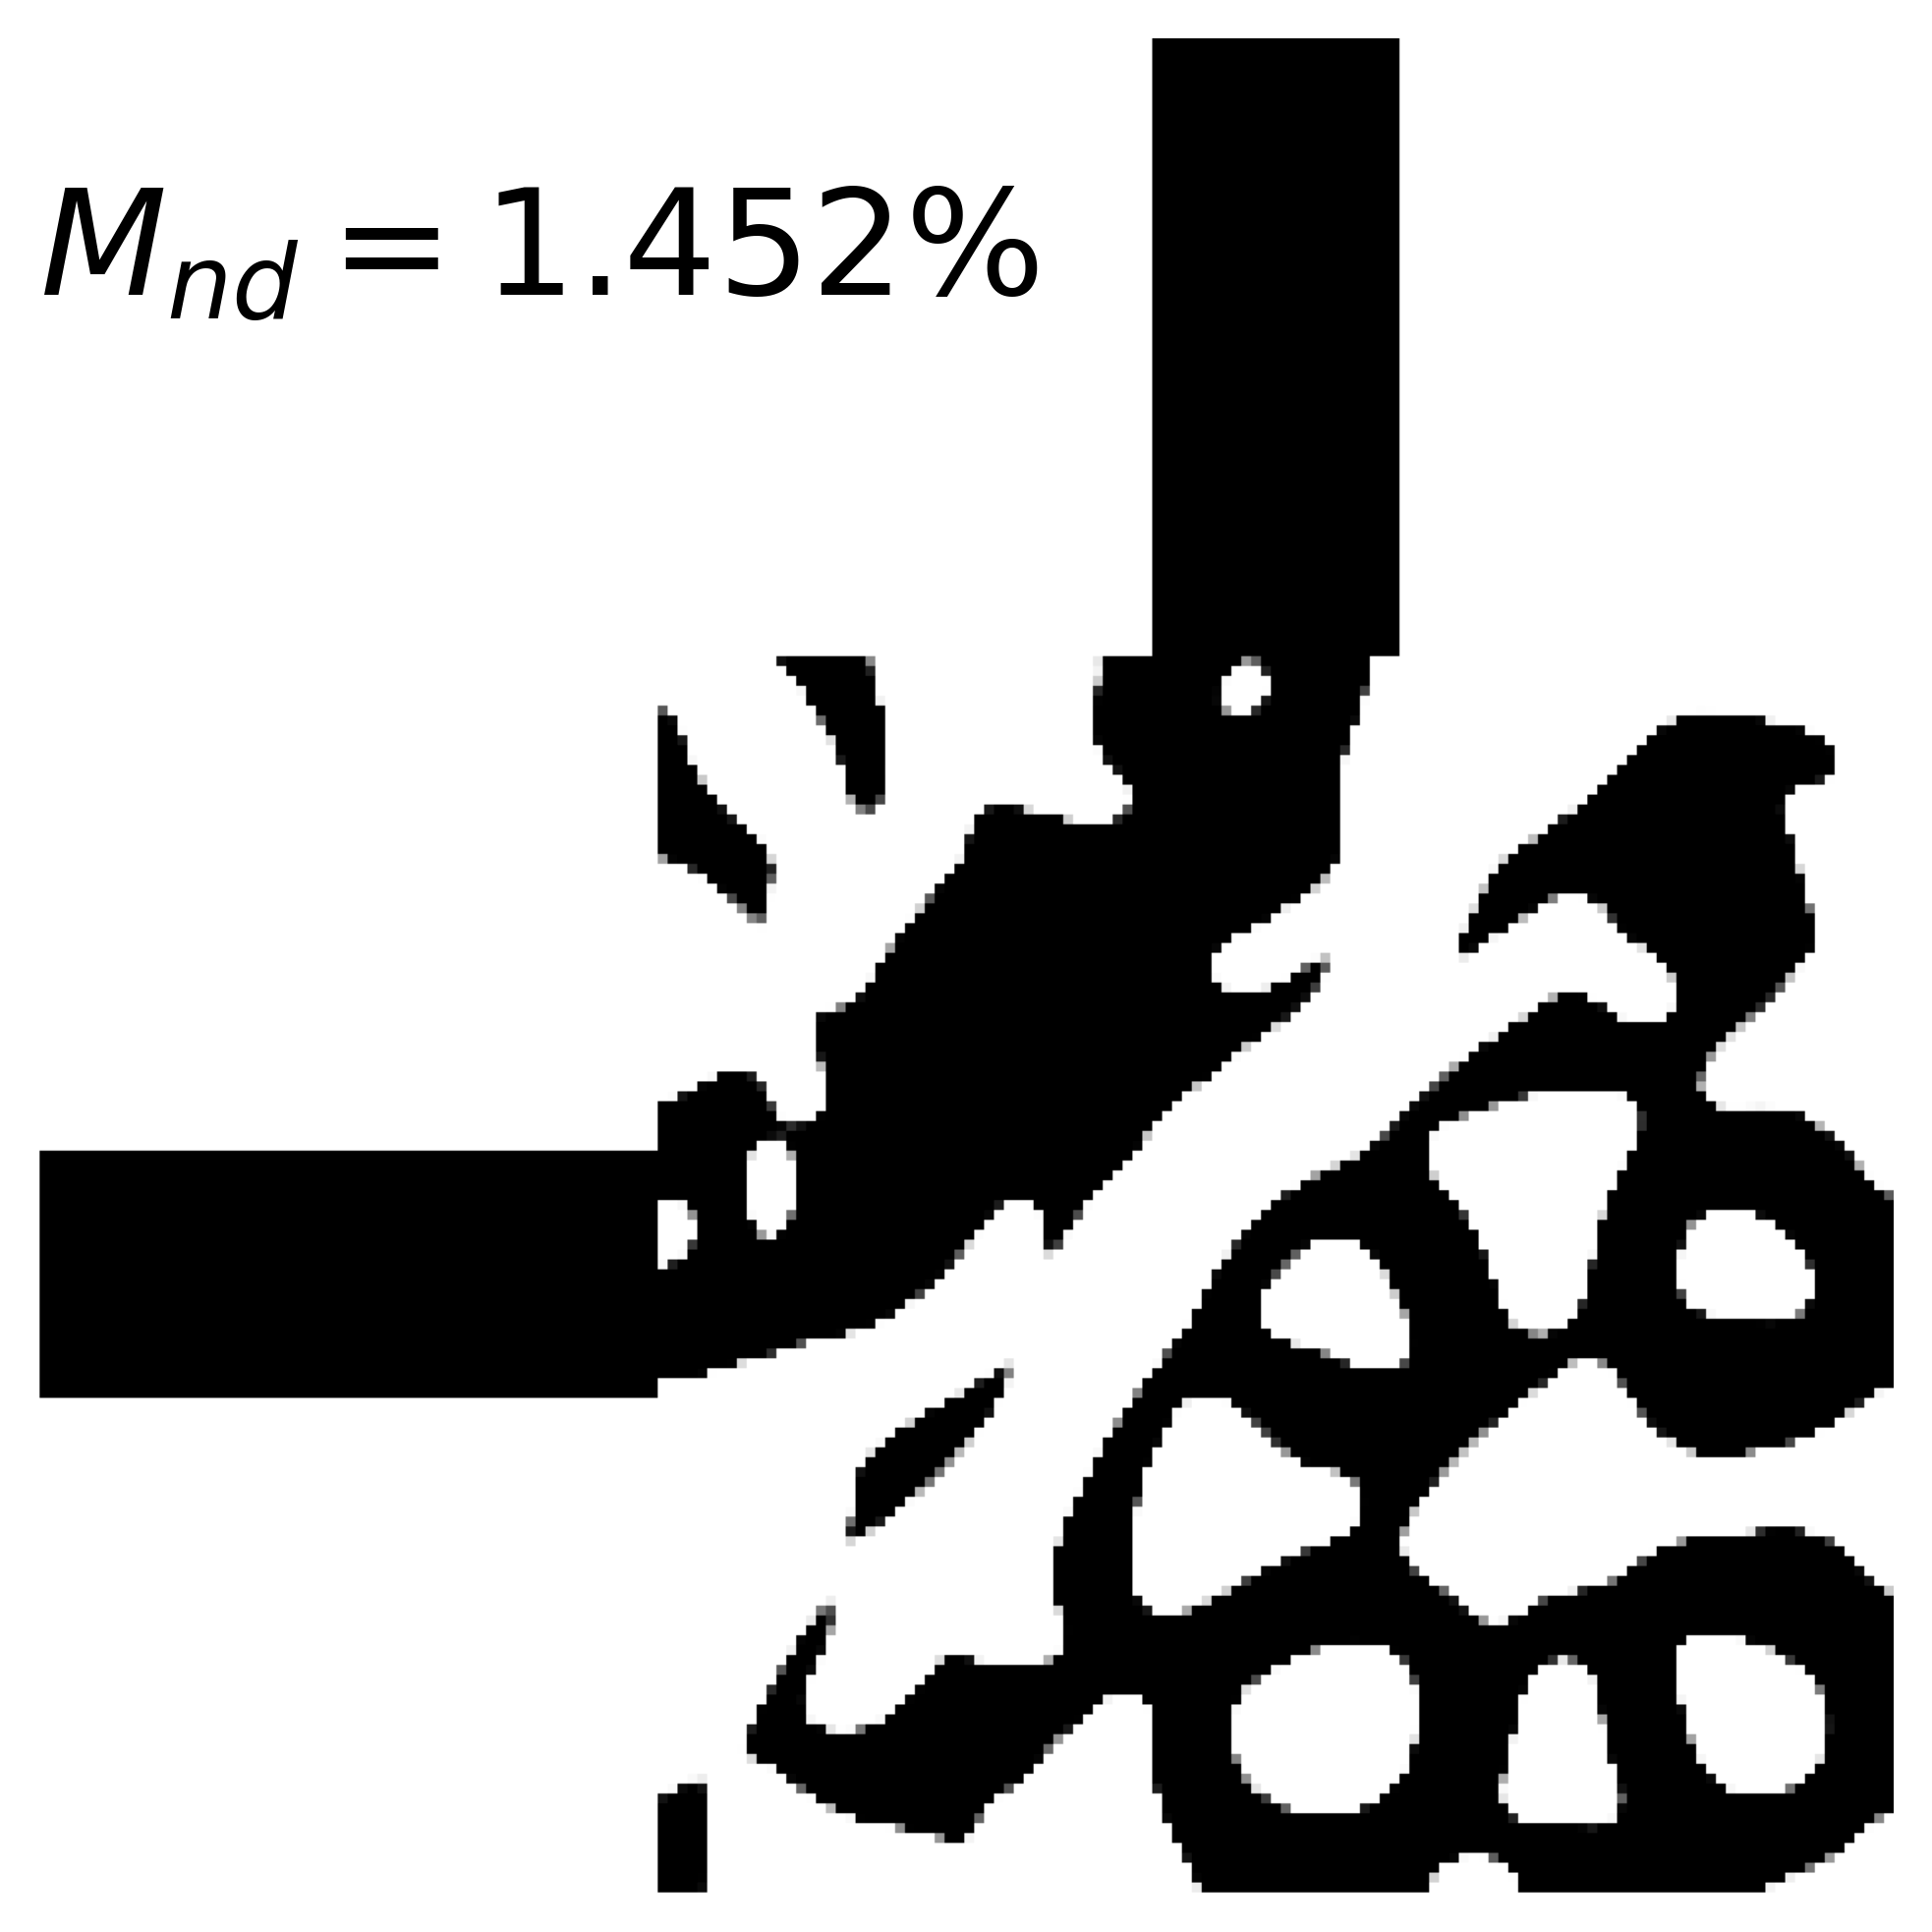
\includegraphics[width=0.3\textwidth]{image/theory/P_E_E.png}\label{subfig:P_E_E}}

  \caption{Aplicación del filtro de densidad y proyección a una parametrización $\boldsymbol{P}.$}
  \label{fig:three-filters}
\end{figure}

Con el objetivo de visualizar estas transformaciones, observemos la \autoref{fig:three-filters}.
En la Figura \autoref{subfig:P} se muestra el diseño que representa una parametrización $\boldsymbol{P}$.
A su derecha se encuentra la Figura \autoref{subfig:P_filter}, aquí se aplicó el filtro de densidad
utilizando un radio de curvatura $r_f = 80 nm$. Como podemos observar, este diseño posee regiones grises,
mas ha logrado eliminar zonas punteagudas.
Seguidamente, en las Figuras \autoref{subfig:P_E_D}, \autoref{subfig:P_E_I}, \autoref{subfig:P_E_E}
se muestra el diseño de la Figura \autoref{subfig:P_filter} tras aplicar la proyección descrita con
$\beta = 2^6$ y distintos valores de $\eta$.
Al utilizar $\eta = \eta_i = 0.5$ (Figura \autoref{subfig:P_E_I}) 
estamos simplemente discretizando el diseño.
Por otro lado, al usar $\eta = \eta_d = 0.3$ (Figura \autoref{subfig:P_E_D})
estamos simulando que el diseño se ha dilatado 
(i.e. la región de $Si$ del diseño intenta expandirse).
Finalmente, al usar $\eta = \eta_e = 0.7$ (Figura \autoref{subfig:P_E_E})
estamos simulando que el diseño ha erosionado 
(i.e. la región de $SiO_2$ del diseño intenta expandirse).


Así, observamos como la proyección presentada en esta sección no solo nos permite discretizar diseños,
sino también simular una dilatación o erosión de estos.
Particularmente, la optimización topológica se considera robusta cuando
tiene en cuenta estas dos posibles modificaciones en el proceso de optimización.
Por otro lado, del mismo modo que se aplicó en la \autoref{fig:three-filters}, para poder diferenciar 
el uso de $\eta$ denotaremos como $\eta_i$ al valor usado en un diseño nominal, 
$\eta_e$ para los diseños erosionados y $\eta_d$ para los diseños dilatados.
Además, es importante señalar que se suele escoger los valores de $\eta_e$ y $\eta_d$
de las manera que $\eta_d = 1 - \eta_e$.
Por último, notemos que  estos parámetros deben seleccionarse con cuidado; 
caso contrario, el diseño podría simular una dilatación o erosión muy exageradas.

Un último punto a considerar es que nuestro proceso de optimización necesitará calcular 
$\nabla f_{obj}(\boldsymbol{P})$, pero al aplicar estas transformaciones terminaremos calculando
$\nabla f_{obj}(\widetilde{\widetilde{\boldsymbol{P}}})$.
Para solucionar este problema podemos implementar las transformaciones presentadas 
de manera que aprovechen la diferenciación automática (similar a lo realizado en la implementación
de MEEP \citep{Oskooi2010}); sin embargo, en el presente trabajo optamos por un enfoque más sencillo
que consiste en utilizar la \autoref{eq:densityfiltergrad} y la \autoref{eq:projection-grad} 
para realizar el cálculo utilizando lo siguiente:

\begin{equation}
  \frac{\partial f_{obj}}{\partial \boldsymbol{P}(x, y)} = \displaystyle\sum_{(x', y') \in \overline{B}_{r_f}(x, y)}
  \frac{\partial f_{obj}}{\partial \widetilde{\widetilde{\boldsymbol{P}}}(x', y')}
  \frac{\partial \widetilde{\widetilde{\boldsymbol{P}}}(x', y')}{\partial \widetilde{\boldsymbol{P}}(x', y')}
   \frac{\partial \widetilde{\boldsymbol{P}}(x', y')}{\partial \boldsymbol{P}(x, y)}.
  \label{eq:fobjgrad}
\end{equation}

Para finalizar esta sección, se presenta una función para medir la presencia de regiones grises.
Esta función ($M_{nd}$) nos ayudará en la evaluación de los diseños optimizados obtenidos en esta tesis,
si obtenemos un valor menor al 2 \% podremos decir que nuestro diseño ha sido correctamente binarizado.

\begin{equation}
  M_{nd} (\boldsymbol{P}) = \frac{\sum_{1 \leq x \leq n \land 1 \leq y \leq m}
  4 \boldsymbol{P}(x, y)(1 - \boldsymbol{P}(x, y))}{n \times m} \times 100 \%.
\label{eq:grayscale}
\end{equation}

Una discusión más detallada de todo lo explicado en esta sección se puede encontrar en \cite{Lazarov2016}.

\section{Algoritmos de Optimización}\label{sec:alg-opt}

Finalmente, con todo lo descrito en este capítulo, ya tenemos las herramientas necesarias
para plantear la optimización de nuestros dispositivos.
Ahora, notemos que nuestro problema se termina reduciendo a maximizar $f_{obj}$.
Sin pérdida de generalidad, en la presente sección se describen algoritmos
para minimizar la función $f = -f_{obj}$.
Esto es posible ya que maximizar una función es equivalente a minimizar su negativo \citep{Mykel2019}.


Para minimizar la función $f$, sea $\pmb{\mathscr{P}}$ el conjunto de todas las matrices 
$\boldsymbol{P}: [1, n] \times [1, m] \to [0, 1]$, queremos encontrar algún mínimo global 
$\boldsymbol{P^{*}} \in \pmb{\mathscr{P}}$, 
donde este elemento se define como una matriz que satisface que
$f(\boldsymbol{P^{*}}) \leq f(\boldsymbol{P}), \quad \forall \boldsymbol{P} \in \pmb{\mathscr{P}}$. 
Dicho de otra manera, nuestro problema es encontrar $\boldsymbol{P^{*}}$; sin embargo,
esto es una tarea computacionalmente dificil de resolver \citep{Angeris2021}.

Un problema más viable es encontrar $\sigma > 0 \land \boldsymbol{P^{+}} \in \pmb{\mathscr{P}}$ 
tal que 
$f(\boldsymbol{P^{+}}) \leq f(\boldsymbol{P}), \quad \forall \boldsymbol{P} \in \pmb{\mathscr{P}}:
|| \boldsymbol{P} - \boldsymbol{P^{+}}|| < \sigma$.
Es decir, es más práctico encontrar $\boldsymbol{P^{+}}$ (conocido como mínimo local)
el cual es un elemento que es un mínimo global si restringimos el espacio de búsqueda a cierta región
alrededor de este elemento.

Debemos resaltar que ninguno de los algoritmos de esta sección puede asegurar encontrar el mínimo global;
sin embargo, sus estrategias de búsqueda suelen permitir encontrar 
óptimos locales adecuados \citep{Angeris2021, Schneider2019}.
Además, todos estos algoritmos se aseguran de mantener los valores de $\boldsymbol{P}$ en el
intérvalo $[0, 1]$ aplicando $\boldsymbol{P}(x, y) \gets max(0, min(1, \boldsymbol{P}(x, y)))$, mas
este detalle se obvia en las explicaciones por simplicidad en la notación.

\subsection{\emph{Genetic Algorithms} (GA)}\label{sec:ga}

Como se describe en el Algoritmo \ref{alg:GA} \citep{Mykel2019}, la idea es 
comenzar generando una población (\emph{population}) de tamaño $population\_size$.
Esta población es un conjunto de matrices de $n \times m$ generadas a partir de una parametrización
inicial $\boldsymbol{P}$, línea 1.
Los siguientes tres pasos se ejecutan por $k$ iteraciones.
Primero, se realiza un proceso de selección para obtener las mejores parametrizaciones
(\emph{parents}), línea 3.
Segundo, los seleccionados se encargan de producir la nueva generación
(\emph{children}), línea 4.
Tercero, la nueva generación muta obteniendo nuevas características, línea 5.

\begin{algorithm}
%\footnotesize
\KwData{$\boldsymbol{P}, population\_size, GA\_range, n\_selected\_parents, prob\_mutation$}
\KwResult{$min(population)$}
$population = generate\_population()$ \\
\For{$t = 0; \, t < k; \, t$++}{
    $parents = select(population)$ \\
    $children = crossover(parents)$ \\
    $population = mutation(children)$
}
\caption{\emph{Genetic Algorithms} (GA)}
\label{alg:GA}
\end{algorithm}

Como se observa en el Algoritmo \autoref{alg:GA}, tenemos las siguientes funciones:

\begin{itemize}
    \item $generate\_population():$ 
      retorna $population\_size$ matrices 
      $\boldsymbol{P'}$ tal que 
      $|\boldsymbol{P'}(x, y) - \boldsymbol{P}(x, y)| \in U(-GA\_range, GA\_range), \quad \forall x \in [1, n]
      \land y \in [1, m]$.

    \item $select(population):$ 
      retorna $n\_selected\_parents$ elementos de $population$ de
      acuerdo a la probabilidad $prob_i$ dada por la ecuación
    
    \begin{equation}
      prob_i = \frac{max(f) - f^{(i)}}{\displaystyle\sum_{j} max(f) - f^{(j)}},
    \label{eq:prob}
    \end{equation}
    
    donde $f^{(i)}$ representa el valor de $f$ aplicado a la 
    $i-$ésima parametrización de $population$ y $max(f)$ es el máximo
    valor de $f$ al haber sido aplicado a todas las matrices de $population$.
    
    \item $crossover(parents):$ 
    retorna $population\_size$ nuevas parametrizaciones.
    Cada nueva matriz $\boldsymbol{S}$ es la combinación de dos parametrizaciones aleatorias 
    $\boldsymbol{P_1}$ y $\boldsymbol{P_2}$ seleccionados de $parents$.
    En esta combinación, para cada $x \in [1, n] \land y \in [1, m]$ se define 
    con igual probabilidad que
    $\boldsymbol{S}(x, y) = \boldsymbol{P_1}(x, y)$ o
    $\boldsymbol{S}(x, y) = \boldsymbol{P_2}(x, y)$.

    \item $mutation(children):$ 
      retorna $children$, pero
      a cada elemento de todas estas matrices
      le agrega un valor en $U(-GA\_range, GA\_range)$ con
      probabilidad $prob\_mutation$.

\end{itemize}

\subsection{\emph{Particle Swarm Optimization} (PSO)}\label{sec:pso}

Podemos pensar este algoritmo como un caso especial del Algoritmo \ref{alg:GA}
\citep{Mykel2019}.
La idea es visualizar el $i-$ésimo individuo como una partícula definida por 
su posición ($\boldsymbol{P^{(i)}}$), velocidad ($\boldsymbol{V}^{(i)}$) y 
la mejor posición encontrada por la partícula ($\boldsymbol{P^{(i)}_b}$).
Para nuestro problema la matriz de parametrización representa la posición y
la velocidad es una matriz que guía la exploración a otras parametrizaciones.

La idea principal del algoritmo es que cada particula acumula 
velocidad en una dirección favorable dada por: 
(i) la mejor posición encontrada hasta el momento por esta partícula y 
(ii) la mejor posición encontrada por la población completa.
Como consecuencia, los individuos se pueden mover independientemente de
perturbaciones locales.
Adicionalmente, agregando caminos aleatorios los individuos incorporan
comportamientos impredecibles que puede permitirles encontrar potenciales
mejores elementos. Esta idea se sintetiza en el Algoritmo \ref{alg:PSO}.

\begin{algorithm}
%\footnotesize
\KwData{$\boldsymbol{P}, population\_size, PSO\_range, \omega, c_1, c_2$}
\KwResult{$\boldsymbol{P_b}$}
$population = generate\_population()$ \\
\For{$t = 0; \, t < k; \, t$++}{
    $\boldsymbol{P_b} = select(population)$ \\
    $population = mutation(population, \boldsymbol{P_b})$
}
\caption{\emph{Particle Swarm Optimization} (PSO)}
\label{alg:PSO}
\end{algorithm}

Como se observa en el \autoref{alg:PSO}, tenemos las siguientes funciones:

\begin{itemize}

    \item $generate\_population():$ 
      retorna $population\_size$ matrices 
      $\boldsymbol{P'}$ tal que 
      $|\boldsymbol{P'}(x, y) - \boldsymbol{P}(x, y)| \in U(-PSO\_range, PSO\_range), \quad \forall x \in [1, n]
      \land y \in [1, m]$. Además genera las matrices $V$ con valores en $U(0, 1)$.

\item $select(population):$ retorna el individuo con el menor valor de $f$ encontrado hasta el momento.

\item $mutation(population, \boldsymbol{P_b}):$ Aplica las siguientes transformaciones a \emph{population}: 
    
  \begin{equation}
    \boldsymbol{P^{(i)}} \gets \boldsymbol{P^{(i)}} + \boldsymbol{V^{(i)}},
  \label{pso-pos}
  \end{equation}

  \begin{equation}
    \boldsymbol{V^{(i)}} \gets \omega \boldsymbol{V^{(i)}} + \
                          c_1 r_1 \left(\boldsymbol{P_{b}^{(i)}} - \boldsymbol{P^{(i)}} \right) + \
                          c_2 r_2 \left(\boldsymbol{P_{b}} - \boldsymbol{P^{(i)}} \right),
  \label{pso-speed}
  \end{equation}
    

  donde $\boldsymbol{P_{b}}$  es la mejor posición encontrada globalmente, 
  $\omega$ representa la tendencia de la particula de conservar su velocidad actual,
  $c_1$ y $c_2$ cuantifica la atracción relativa con $\boldsymbol{P_{b}^{(i)}}$ y 
  $\boldsymbol{P_{b}}$ respectivamente, 
  y $r_1, r_2 \in U(0, 1)$ representan el comportamiento impredecible.

\end{itemize}

\subsection{\emph{Covariance Matrix Adapatation Evolution Strategy} (CMA-ES)}\label{sec:cma-es}

La idea general de esta estrategia evolutiva, mostrada en el Algoritmo
\ref{alg:CMA}, es mantener:
(i) un vector $\boldsymbol{\mu}$ $p$-dimensional,
(ii) una matriz $\boldsymbol{C}$ y
(iii) un número $\sigma$ para ir generando $n$ inviduos $p$-dimensionales
a partir una distribución $\mathcal{N}(\mu,\,\sigma^{2} \boldsymbol{C})$.


Tomar puntos de esta distribución limita el espacio de búsqueda a una
hiperelipse.
Así, el algoritmo evalua puntos en esta región limitada.
Luego, usando los valores obtenidos, se puede decidir entre:
(i) mover la hiperelipse a otra región del espacio de búsqueda
(ii) expandir or reducir la región cubierta por la distribución.
El algoritmo de CMA-ES trabaja iterativamente sobre esta idea hasta que la
hiperelipse termina casi degenerándose en un punto, 
potencialmente un óptimo.

\begin{algorithm}
  \KwData{$\boldsymbol{P}, population\_size, \sigma$}
\KwResult{$\boldsymbol{\mu}$}
$\boldsymbol{\mu} = flatten(\boldsymbol{P})$ \\
\For{$t = 0; \, t < k; \, t$++}{
  sample() \tcp{Obtener $population\_size$ puntos de $\mathcal{N}(\boldsymbol{\mu},\,\sigma^{2} \boldsymbol{C})$}
    update() \tcp{Ecuación \ref{cma-average}}
    control() \tcp{Ecuación \ref{cma-control}}
    adapt() \tcp{Ecuación \ref{cma-adapt}}
}
\caption{CMA-ES}
\label{alg:CMA}
\end{algorithm}


Entrando en más detalles del Algoritmo \ref{alg:CMA},
en la línea 1 simplemente se linealiza la matriz $\boldsymbol{P}$ en un vector $\boldsymbol{\mu}$ 
de dimensión $p = n \times m$ (i.e. se unen sus vectores filas en orden para formar un solo vector).
Luego, dentro del bucle en la iteración $t$, en la línea 3 se genera $population\_size$ puntos
$p$-dimensionales $\boldsymbol{x_i}$ de la distribución $\mathcal{N}(\boldsymbol{\mu},\,\sigma^{2} \boldsymbol{C})$, 
donde estos son ordenados ascendentemente de acuerdo
al valor de $f$.
En la línea 4 actualizamos la media $\boldsymbol{\mu}$ usando una promedio ponderado dado
por

\begin{equation}
  \boldsymbol{\mu^{(t + 1)}} \gets \sum_{i=1}^{n} w_i \boldsymbol{x_i},
\label{cma-average}
\end{equation}

donde $w_i$ son valores fijos y escogidos de tal manera que proporcionen mayor
contribución a los puntos con menor valor al evaluarlos en $f$. 
Esto permite mover la media $\boldsymbol{\mu}$ en una dirección favorable.

Seguidamente, se necesita actualizar $\sigma$ para expandir o reducir la
hiperelipse en la siguiente iteración. Por este motivo, la línea 5 controla
este valor mediante las ecuaciones

\begin{equation}
    \sigma^{(t + 1)} \gets \sigma^{(t)} \exp\bigg(\frac{c_{\sigma}}{d_{\sigma}}
    \underbrace{\left(\frac{||\boldsymbol{p_{\sigma}}||}{\mathbb{E}||\mathcal{N}(0,
    \mathbf{I})||} - 1 \right)}_{\text{evolution path comparison}} \bigg),
\label{cma-control}
\end{equation}

\begin{equation}
\mathbb{E}||\mathcal{N}(0, \mathbf{I})|| = \sqrt{2} \left(
  \frac{\Gamma\left(\frac{p + 1}{2}\right)}{\Gamma\left({\frac{p}{2}}\right)}
  \right),
\label{cma-E}
\end{equation}

donde $\boldsymbol{p_{\sigma}}$ es una variable que acumula los pasos llevados,
$c_{\sigma} \in [0, 1]$ es una variable que determina el tiempo acumulado para $p_{\sigma}$ y 
$d_{\sigma} \approx 1$ es un parámetro que determina el ratio de posibilidad de cambio de $\sigma^{(t + 1)}$. 
La principal parte de la \autoref{cma-control} es el término \emph{evolution path comparison}, 
aquí se compara el tamaño de $p_{\sigma}$ con su tamaño esperado bajo selección
aleatoria.
De esta comparación podemos controlar si el valor de $\sigma$ debe
incrementarse, disminuirse o permanecer igual.

Finalmente, en la línea 6 cambiamos $\boldsymbol{C}$ a una dirección favorable usando lo siguiente:

\begin{multline}
  \boldsymbol{C^{(t + 1)}} \gets \overbrace{\bigg(1 - c_1 c_c (1 - h_{\sigma})(2 - c_c) - c_1 - c_{\mu}\bigg) \boldsymbol{C^{(t)}}}^{\text{cumulative update}} \\
    + \underbrace{c_{1} \boldsymbol{p_{C}} \boldsymbol{p_{C}}^{T}}_{\text{rank-one update}}
    + \underbrace{c_{\mu}\sum_{i=1}^{n}w'_{i}
    \boldsymbol{\delta^{(i)}}\left(\boldsymbol{\delta^{(i)}}\right)^{T}}_{\text{rank-}\mu\text{ update}},
\label{cma-adapt}
\end{multline}

donde $c_{\mu} \leq 1$ es el radio de aprendizaje para el término \emph{rank-$\mu$ update}, 
$c_1 \leq 1 - c_{\mu}$ es el radio de aprendizaje para el término \emph{rank-one update}, 
$c_c \in [0, 1]$ es el radio de aprendizaje para el término \emph{cumulative update}, 
$h_{\sigma}$ es la evaluación bajo la función unitaria usado para actualizar
apropiadamente el camino evolutivo, 
$\boldsymbol{p_{C}}$ es un vector acumulativo usado para actualizar la matriz de
covarianza, 
$w'_i$ son los coeficientes de ponderación modificados y
$\boldsymbol{\delta^{(i)}}$ son las desviaciones seleccionadas.

En la \autoref{cma-adapt}, el primer término (\emph{cumulative update}) 
mantiene información de la anterior matriz de convarianza.
El segundo término (\emph{rank-one update}) permite expandir la distribución en
una dirección favorable.
El tercer término (\emph{rank-$\mu$ update}) incrementa la búsqueda en espacios
donde es probable encontrar buenas soluciones.
La combinación de estos tres términos actualiza $\boldsymbol{C}$ de tal manera que
mueva la hiperelipse en una dirección favorable. 
Para una descripción más detallada del algoritmo, revisar los trabajos de \cite{Hansen2016} y \cite{Mykel2019}.

\subsection{\emph{Gradient Descent} (GD)}\label{sec:gradient-descent}

Este algoritmo comienza desde un punto inicial, en nuestro caso la matriz $\boldsymbol{P}$.
Luego, usa la derivada en ese punto para guiar su búsqueda iterativamente, 
esto lo realiza mediante la siguiente ecuación:

\begin{equation}
  \boldsymbol{P^{(t+1)}} \gets \boldsymbol{P^{(t)}} - \gamma \nabla \boldsymbol{P^{(t)}},
  \label{eq:gd-point}
\end{equation}

donde $t$ representa la iteración actual y $\gamma$ (conocido como el ratio de aprendizaje)
determina la magnitud de como actualizar $\boldsymbol{P^{(t)}}$. 
Particularmente, un enfoque razonable para buscar convergencia a 
un mínimo local es actualizar $\gamma$ en cada iteración mediante la ecuación

\begin{equation}
  \gamma^{(t+1)} = \frac{|(\boldsymbol{P^{(t)}}-\boldsymbol{P^{(t-1)}})^T(\nabla f(\boldsymbol{P^{(t)}})-\nabla f(\boldsymbol{P^{(t-1)}}))|}
  {||\nabla f(\boldsymbol{P^{(t)}})-\nabla f(\boldsymbol{P^{(t-1)}})||^2}.
  \label{eq:gd-gamma}
\end{equation}

Un detalle importante a señalar es que por simplicidad en la notación, 
la \autoref{eq:gd-gamma} se describió de esta manera;
sin embargo, en realidad debemos trabajar con la matriz $\boldsymbol{P}$ después de ser linealizada
para que las operaciones de esta ecuación estén bien definidas.
Mayores detalles del algoritmo se pueden encontrar en \cite{Demidova2020}.


\subsection{\emph{Method of Moving asymptotes} (MMA)}\label{sec:mma}

\emph{Method of moving asymptotes} (MMA) es un algoritmo de optimización
local basado en la gradiente, es decir, de primer orden.
La idea del algoritmo es comenzar en un punto $\boldsymbol{P}$ y formar
una aproximación de $f$ alrededor de $\boldsymbol{P}$ utilizando:
(i) la gradiente de $f$,
(ii) los límites de los valores de $P$ y
(iii) una función de penalidad cuadrática.
Lo interesante de esta aproximación es que es convexa y separable, lo cual permite
resolverla de forma sencilla.
Así, el algoritmo comienza calculando la aproximación, luego resuelve la optimización
utilizando la aproximación.
De este modo, surgen dos posibles escenarios:
(i) la aproximación encuentra un buen elemento que se usa como punto de inicio para repetir el procedimiento o
(ii) se repite el proceso limitando la contribución de la función de penalidad.

En realidad en el presente trabajo usaremos una versión mejorada del algoritmo
conocida como \emph{Conservative Convex Separable Approximation} (CCSA) 
debido a su popularidad en optimización topológica, pero nos seguiremos refiriendo
al algoritmo como MMA por convención.
Esta variante tiene la particularidad de lograr converger a un mínimo local independientemente
del punto inicial. Los detalles se pueden revisar en \cite{Svanberg2002}.

\subsection{\emph{Limited-memory Broyden–Fletcher–Goldfarb–Shanno with boundaries} (L-BFGS-B)}\label{sec:lbfgsb}

\emph{Limited-memory Broyden–Fletcher–Goldfarb–Shanno with boundaries} (L-BFGS-B) es un algoritmo
de optimización que se caracteriza por estimar la inversa de la matriz hessiana utilizando 
una cantidad de memoria de orden lineal.
El algoritmo comienza con un punto inicial $\boldsymbol{P}$.
Luego, internamente mantiene el historial de las últimas evaluaciones de la función $f$ y $\nabla f$
para determinar una dirección para actualizar $\boldsymbol{P}$.
Esto es posible precondicionando la gradiente con información de curvatura obtenida por
la aproximación de la matriz hessiana.
El lector interesado puede revisar los detalles del algoritmo en \cite{Liu1989}.


En el presente capítulo se ha descrito la teoría necesaria para optimizar el diseño de un
un \emph{bend} y WDM.
Esto ha implicado la explicación de la parametrización basada en píxeles,
el uso de SPINS-B y transformaciones utilizadas en la optimización topológica robusta.
Además, se ha desarrollado la explicación de tres algoritmos que no necesitan calcular la gradiente:
(i) GA, (ii) PSO y (iii) CMA-ES. Asimismo, se describió tres algoritmos de primer orden 
(que usan la gradiente): (i) GD, (ii) MMA y (iii) L-BFGS-B.
Los conceptos presentados serán de utilidad para entender la propuesta de esta tesis descrita en el
\autoref{chapter:methodology}.


%\leonidas{Hablar en más detalle de esto y acompañarlo con una imagen de conversión de una curva al 
%formato GDSII similar al paper de Lukas \citep{Bogaerts2018} o hacer mención de esto en los 
%resultados directamente}
